{
Eventually, the dapp took shape thanks to the combination of the technology explained in the previous section. By using the backend on-blockchain, the backend off-blockchain, and the frontend web application, I have built an accessible web app that lets standard users the possibility to contract a car insurance policy with blockchain empowered capabilities, such as ownership and censorship-resistance. The clients can read the policy contract before confirming the purchase and make it clear what the company can and cannot do. All the operations are transparent and there is even a trace of all computations carried out so the blockchain model enhances the situation of the traditional model. The dapp project has been called \textbf{Insurechain}, mixing the words ``blockchain" and ``insurance".


}
\subsection{Dapp software overview}
{
The resulting software stack of the dapp may be cumbersome. It relies on every piece in charge of some specific tasks that combined with the other pieces deliver a comprehensive and valuable product. To have a clear idea of the elements involved we can take a look at the figure \ref{fig:dapp-overview}.

\begin{figure}[H]
\centering
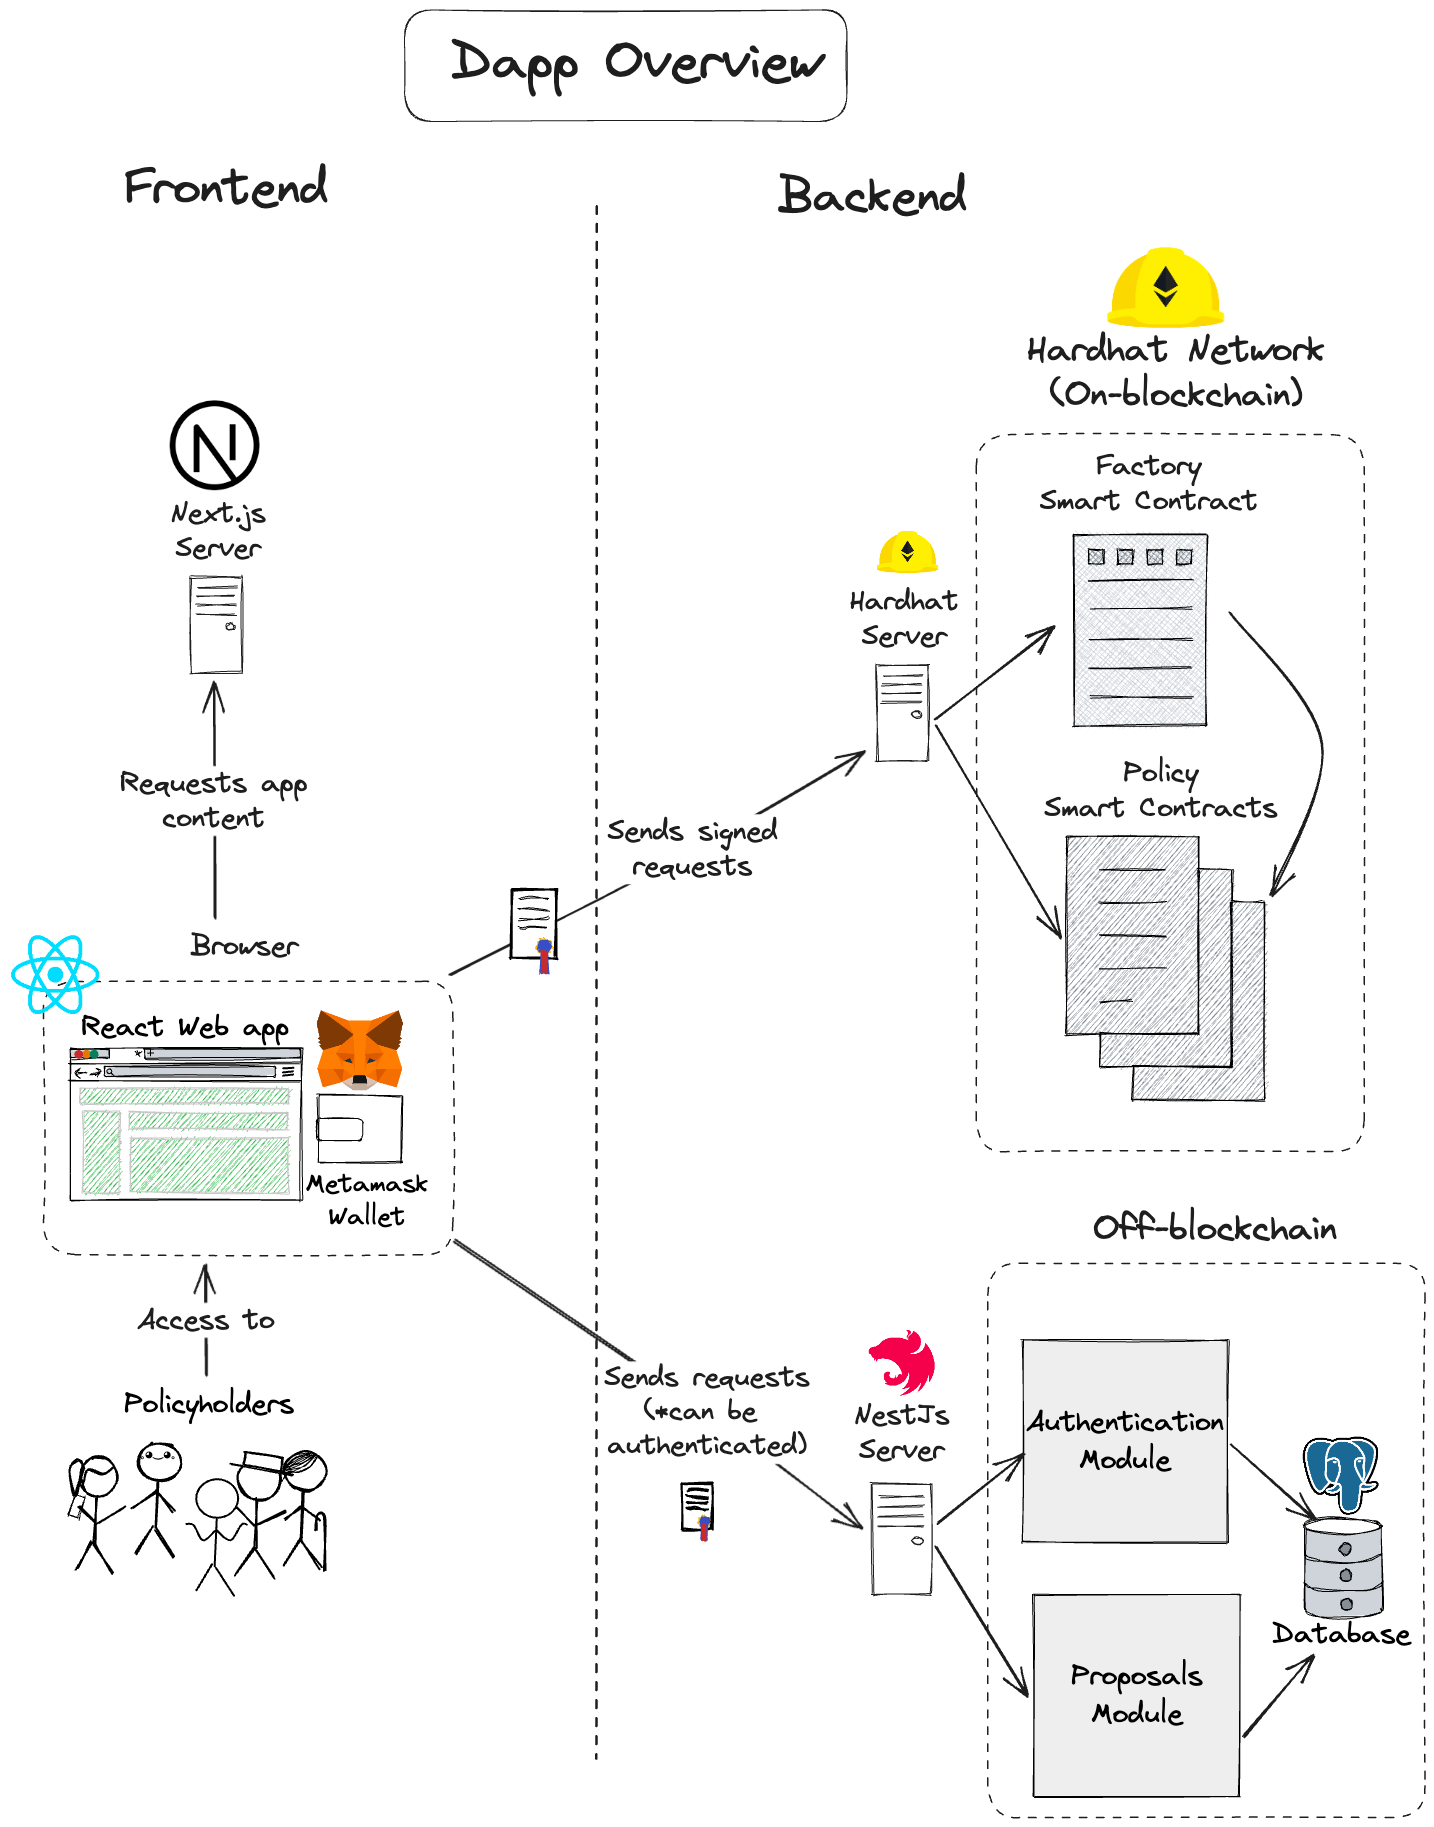
\includegraphics[width=14cm]{img/results/dapp-overview.png}
\caption[Dapp software overview]{\footnotesize{Dapp software overview.}}
\label{fig:dapp-overview}
\end{figure}

There are some insights to highlight in this breakdown:
\begin{itemize}
    \item The policyholders can easily access the dapp through the web app technology and a wallet such as Metamask. The Next.js server is responsible for delivering the UI that the web app demands to display the data properly.
    \item The communication with the backend can be authenticated or not depending on the moment the user signs in using the wallet. This way, the identification of a user is the same for both backend pieces: the user address. Although the Ethereum transactions get signed by protocol automatically, the NestJs server verifies as well the user by the authentication flow based on ``Siwe".
    \item The Nestjs server protects some endpoints according to the need to create data bound to a specific user address. 
    \item The Nestjs modules rely on the relational database to store all the proposals list of the users, where the primary key is their account address. In this manner, we prevent the user from consuming gas, i.e. spending money, just to create a proposal, which from the product point of view does not make any sense. Hence, creating proposals does not have any blockchain effect.
    \item The web application can display all proposals of a user. If a user wants to purchase one, this transaction is emitted to the Hardhat network when the Factory smart contract is deployed. There, it creates and deploys a Policy smart contract and returns the deployment address. Metamask helps the user by displaying the transaction details and prompting them to confirm the execution.
    \item Since the Factory smart contract stores data from all the policies created for each user, every user can get their policy details on the web application. 
    \item The policyholders can perform actions on the policy smart contract. The web app application has implemented the cancel method which requires the minimum computational gas to confirm the transaction.
\end{itemize}

I would like to emphasize that the backend parts do not communicate between them intentionally. Each part is in charge of storing a certain part of the business logic that has been thought for. It is beyond the scope of this experiment to make an interface for the company and evaluators, because it is a matter of fact that converting the policyholder flow proves that the conversion to the blockchain model is feasible from the other parts too since it is streamlining the communication for all parts concerned. Furthermore, from the point of view of the company, it also offers a lot of value since users have to pay to operate over the policy which represents a first barrier for reducing fraud but also there are incredible possibilities to rely on the blockchain such as trust the risk computation to the network so the policyholders cover themselves, therefore the proposal quote price and renewals regulates automatically depending on historical accident rate.
}

\subsection{User experience flows}
{
In this section, we can find the resulting user experience flows of what a policyholder is facing when he opens the Insurechain web application to obtain a car policy. To make explanations more clear and accurate, during this whole section the on-blockchain part is referred to as smart contracts, the off-blockchain part as the backend, and the frontend part as the web app.
}

\subsubsection{Landing page}
{
Every web application has a landing page. This page is where a new user usually "lands". There, he may find all the information about what the product does and which are its benefits. Moreover, the company is introduced to the client. In so doing, the user can make a quick idea about what the company offers to him. For Insurechain, I simulated what could be a landing page, as you may see in figures \ref{fig:landing-1}, \ref{fig:landing-2}, \ref{fig:landing-3} and \ref{fig:landing-4}.
\begin{figure}[H]
\centering
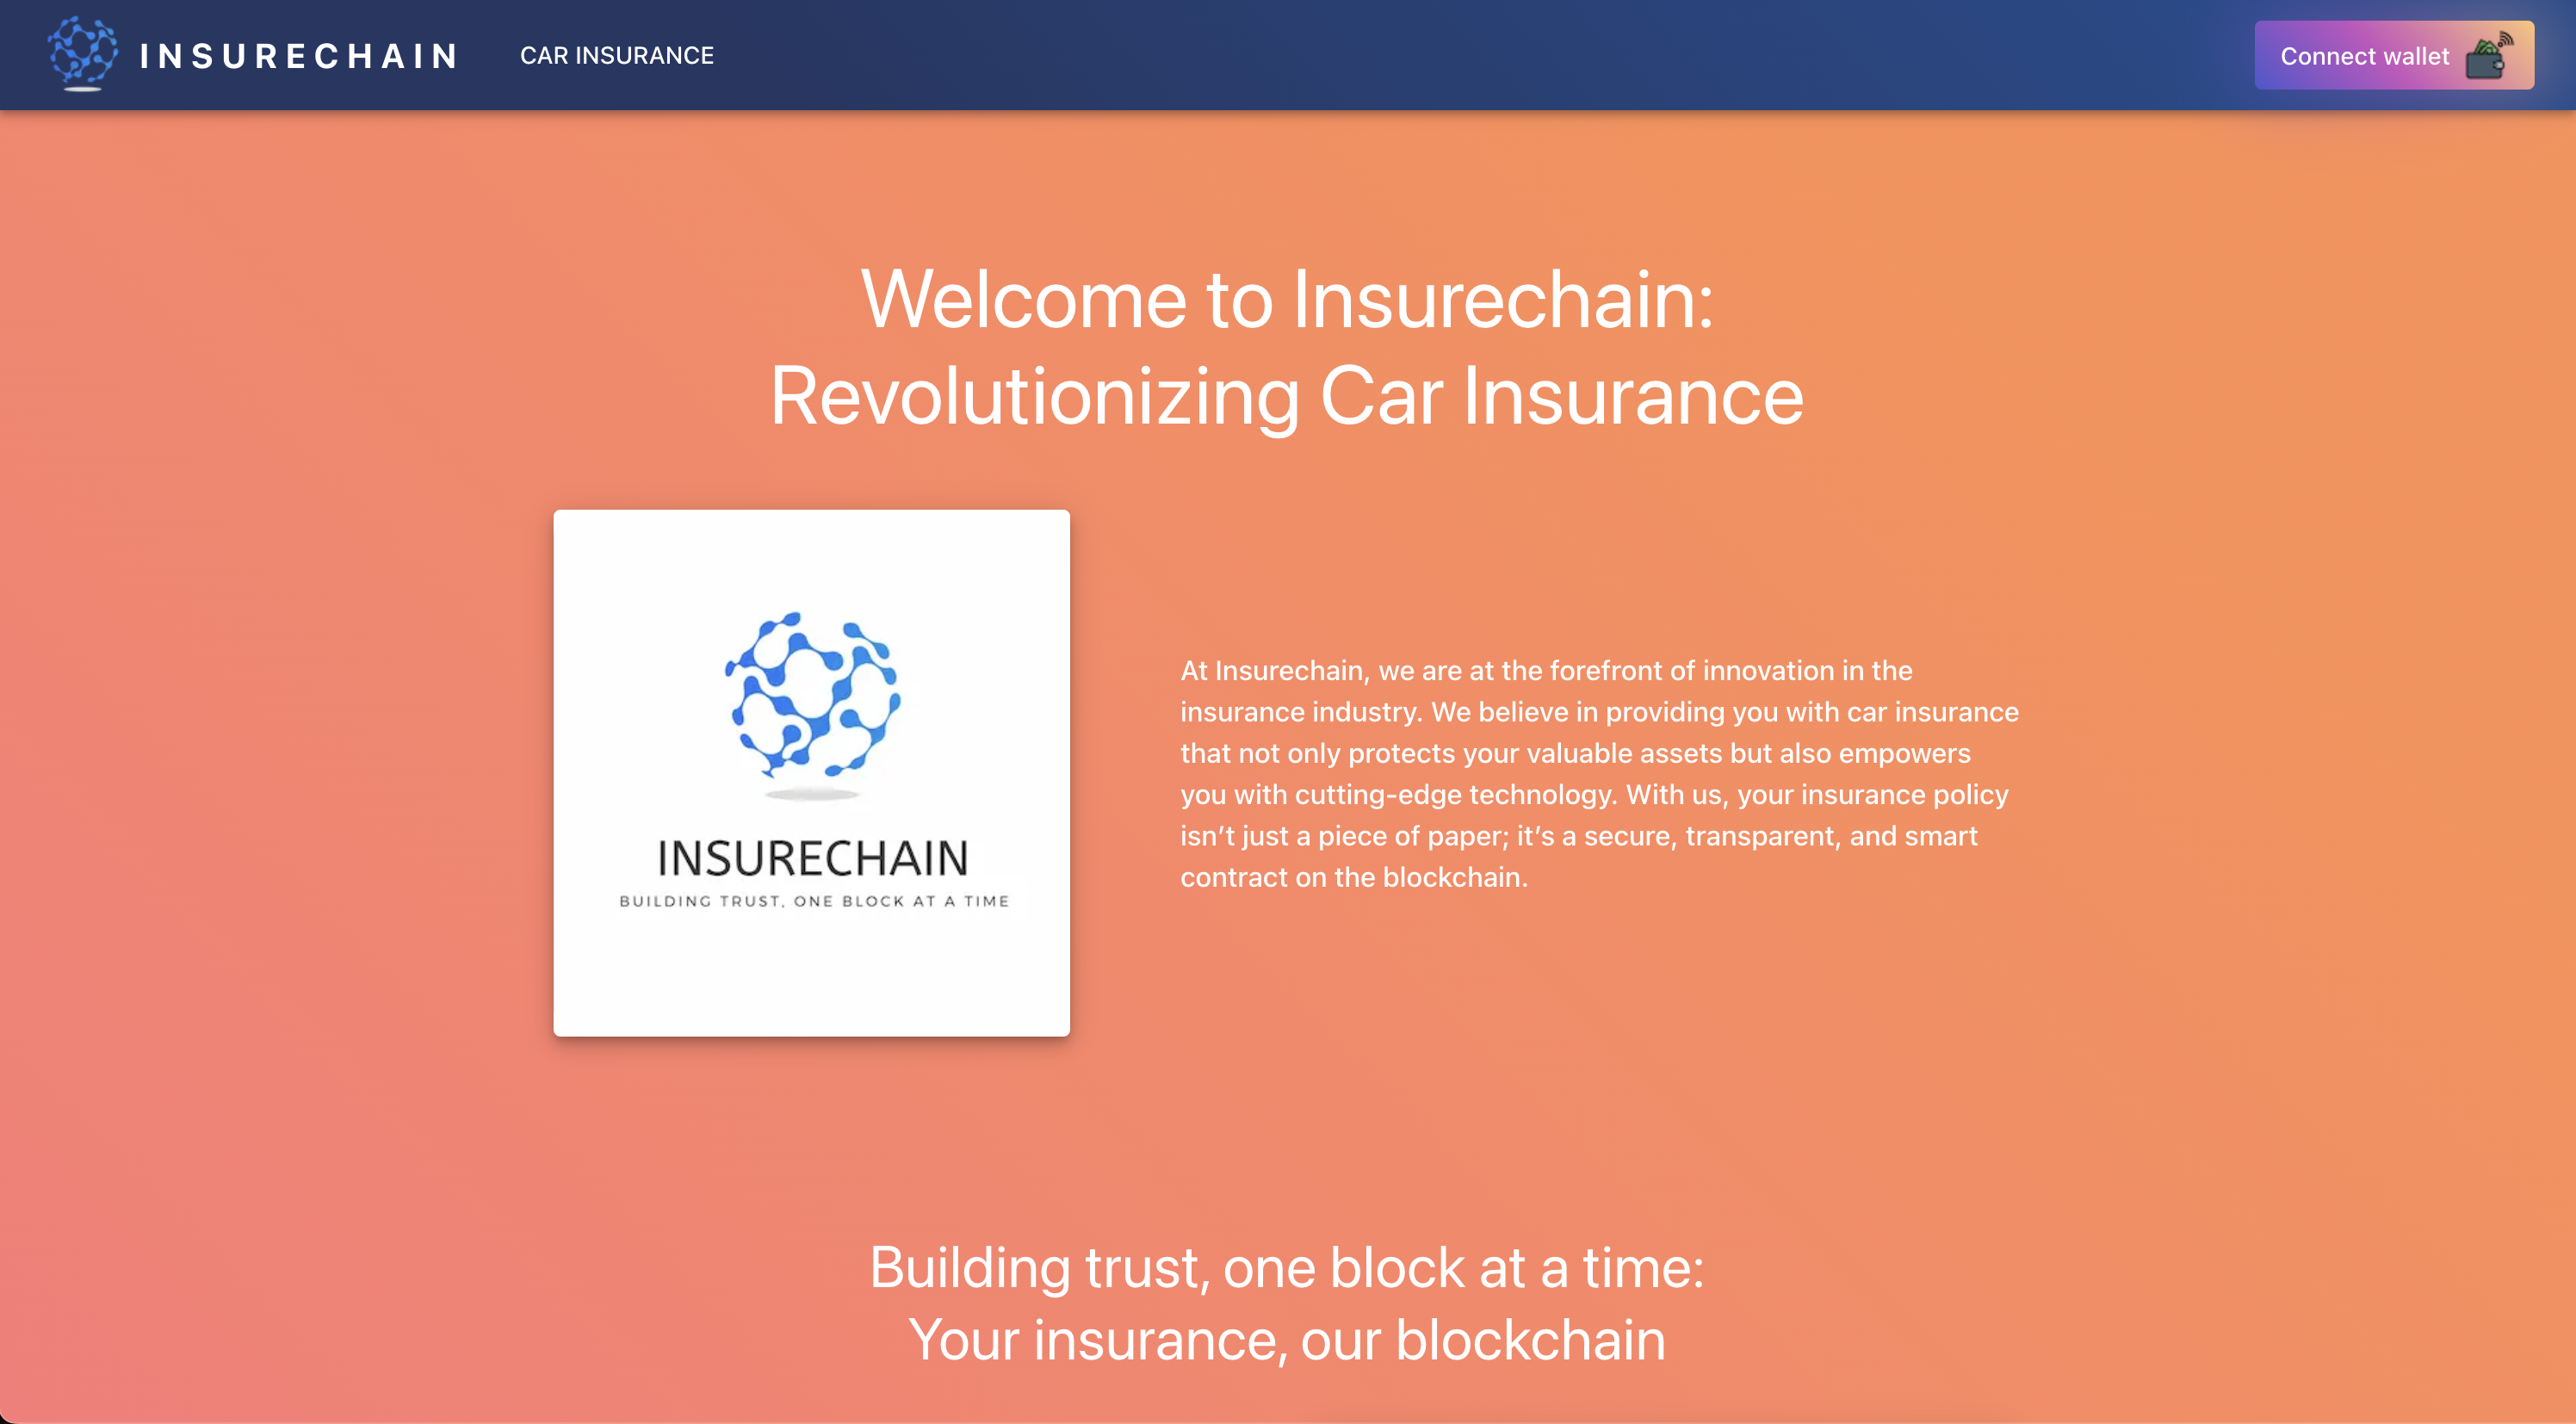
\includegraphics[width=14cm]{img/results/landing-1.png}
\caption[Landing page - part 1]{\footnotesize{Landing page - part 1.}}
\label{fig:landing-1}
\end{figure}

\begin{figure}[H]
\centering
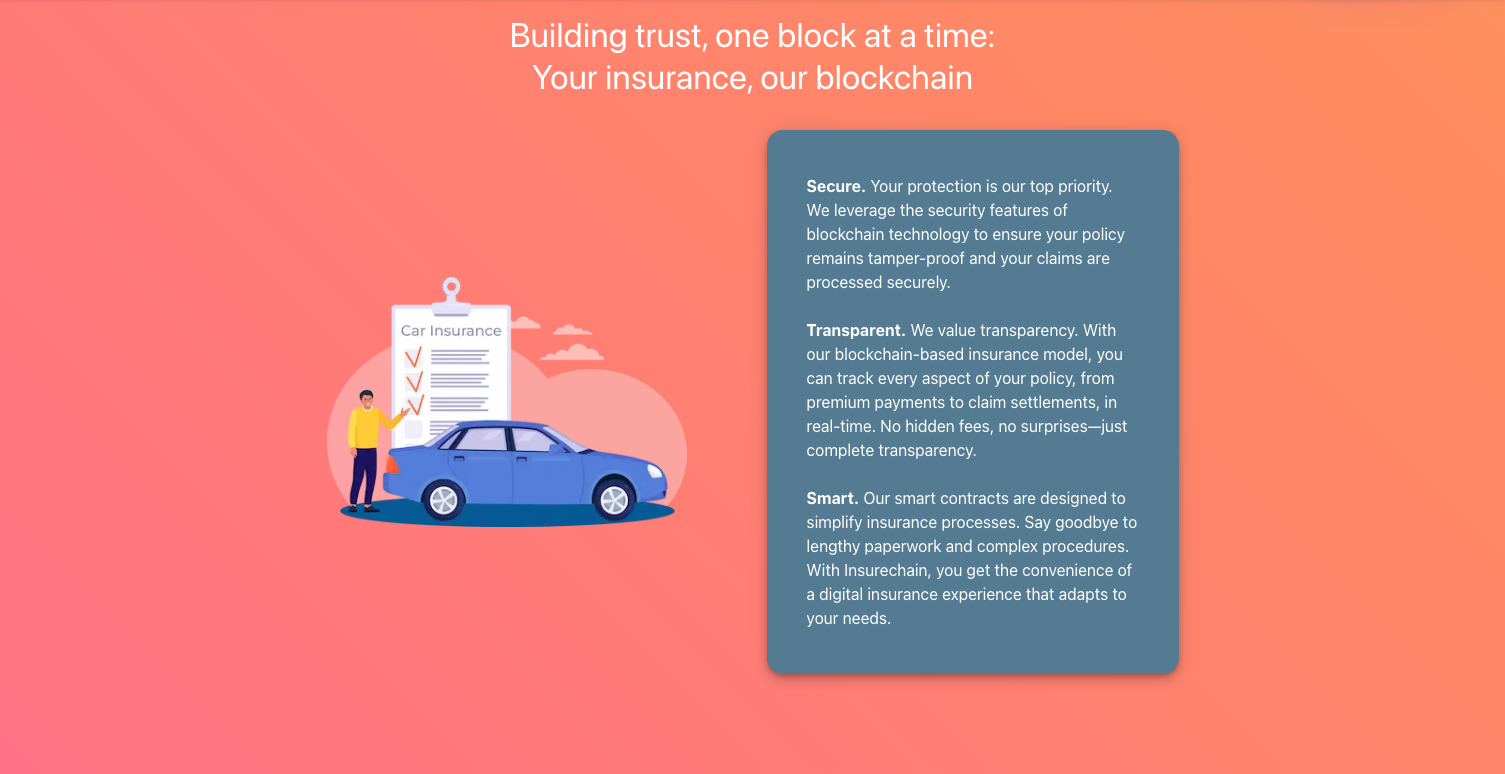
\includegraphics[width=14cm]{img/results/landing-2.png}
\caption[Landing page - part 2]{\footnotesize{Landing page - part 2.}}
\label{fig:landing-2}
\end{figure}

\begin{figure}[H]
\centering
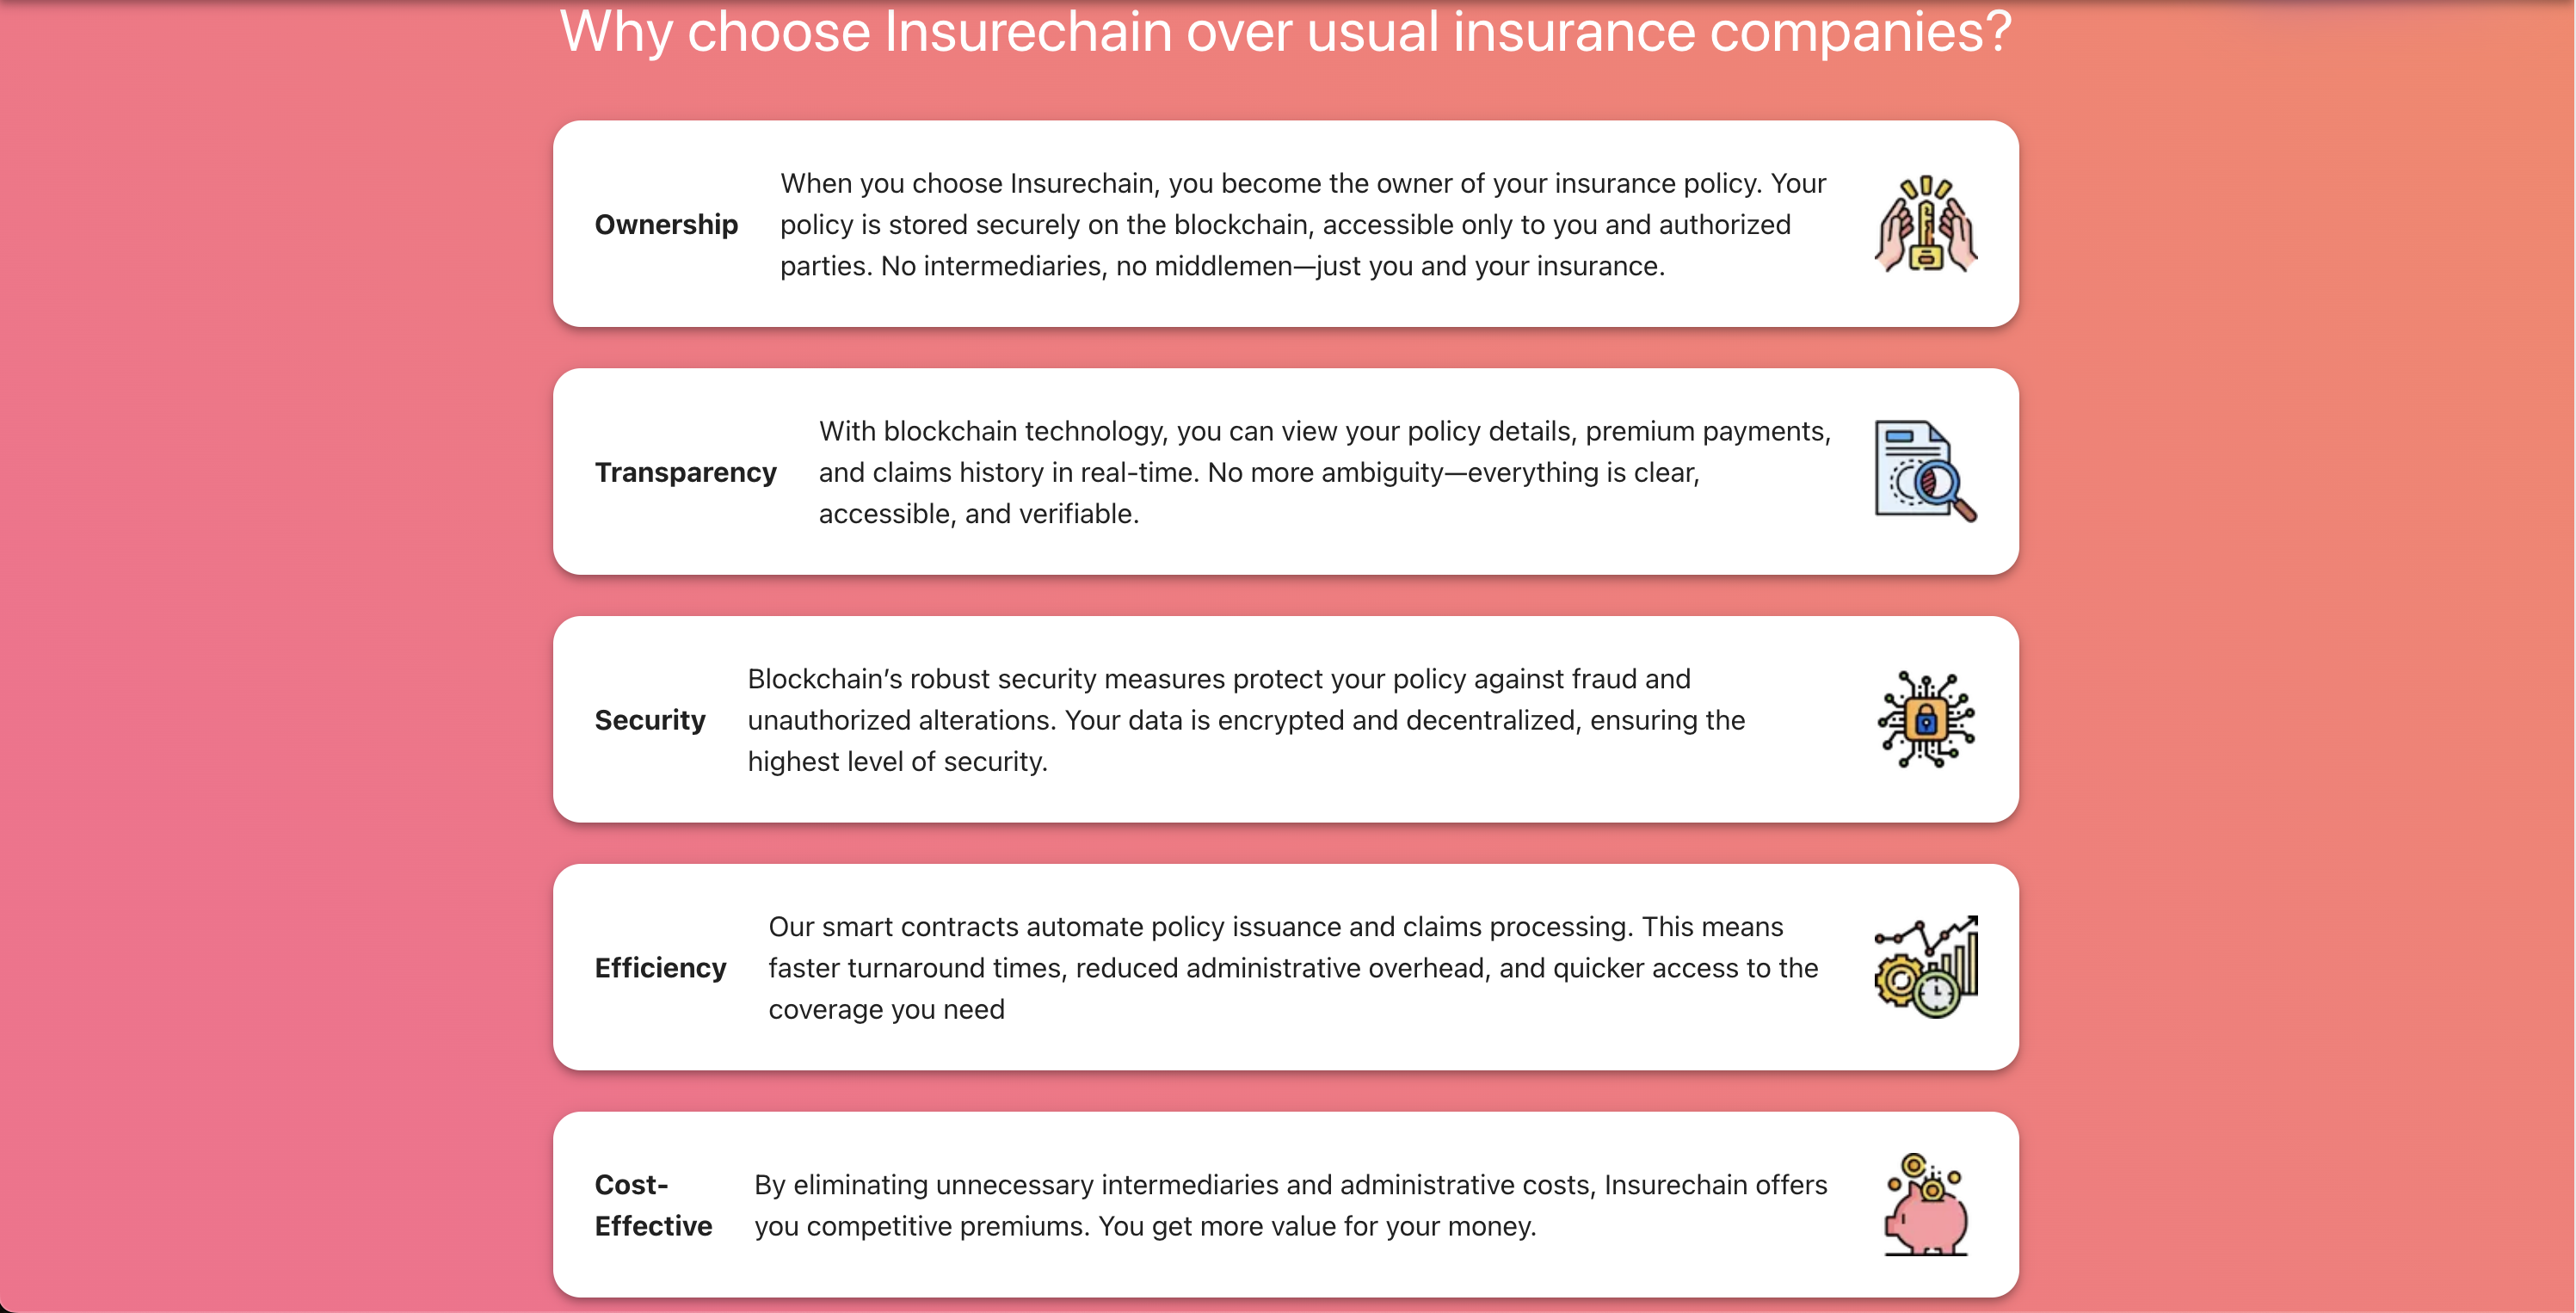
\includegraphics[width=14cm]{img/results/landing-3.png}
\caption[Landing page - part 3]{\footnotesize{Landing page - part 3.}}
\label{fig:landing-3}
\end{figure}

\begin{figure}[H]
\centering
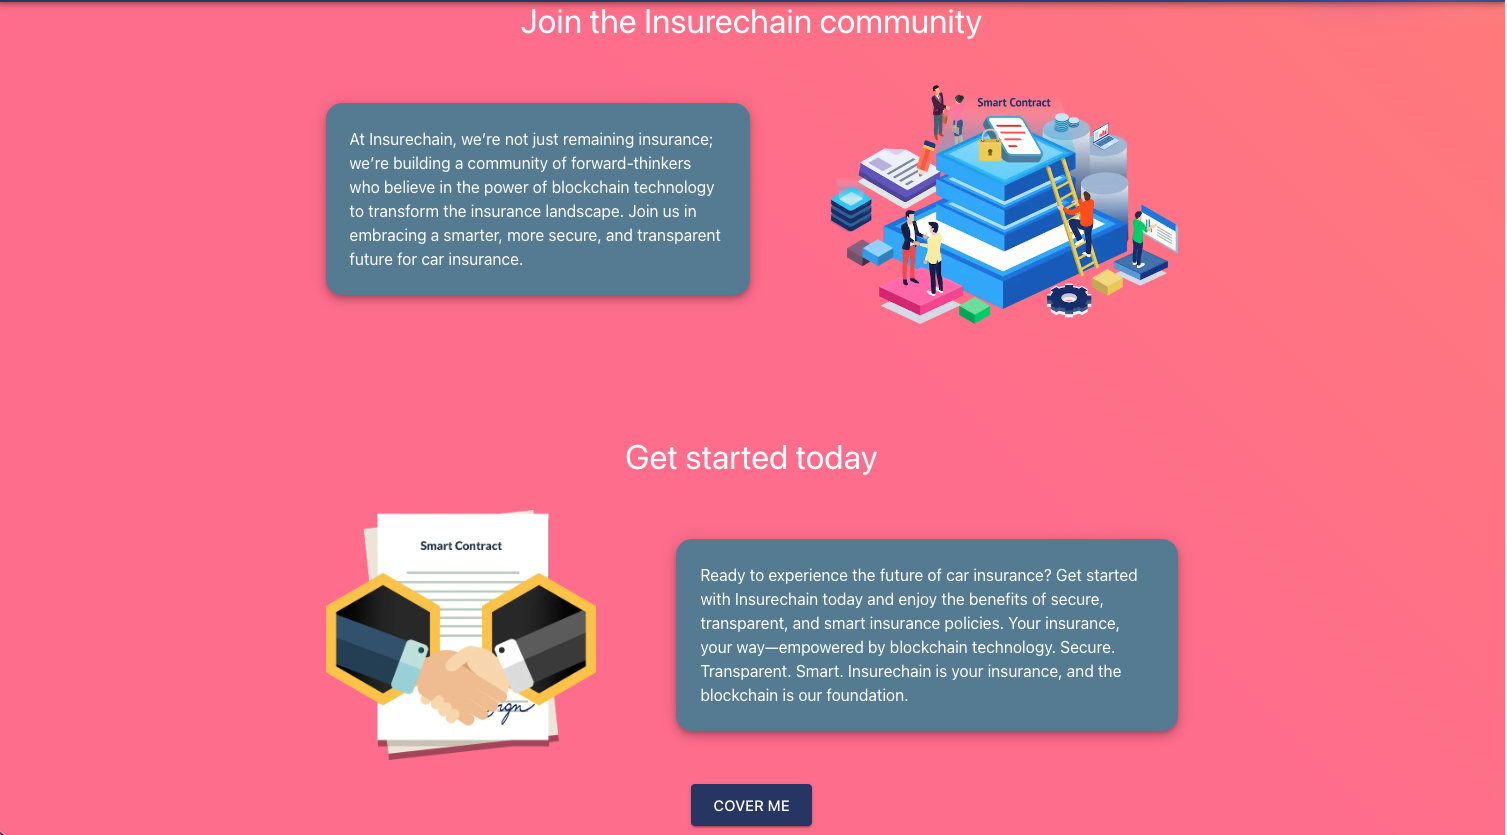
\includegraphics[width=14cm]{img/results/landing-4.png}
\caption[Landing page - part 4]{\footnotesize{Landing page - part 4.}}
\label{fig:landing-4}
\end{figure}

As you may see, there is a basic but comprehensive explanation of what the product achieves and the advantages for the user. Finally, the user can find a ``Call to action" button to begin the process of creating a proposal.
}

\subsubsection{Login}
{
In the header, which is the fixed toolbar located at the top of the page that you can see in figure \ref{fig:header-toolbar}, we may find the Insurechain logo, a link "Car Insurance" which navigates to the Car insurance proposal enrollment. In addition, on the right side, we may find a button that says "Connect Wallet".
\begin{figure}[H]
\centering

\includegraphics[width=14cm]{img/results/header.png}
\caption[Insurechain: Header toolbar]{\footnotesize{Header toolbar.}}

\label{fig:header-toolbar}
\end{figure}

Clicking on the "Connect to wallet" displays the available wallets installed in your browser. Each client is supposed to choose one. In the experiment, we have used Metamask as you may see in figure \ref{fig:wallet-list}. 

\begin{figure}[H]
\centering
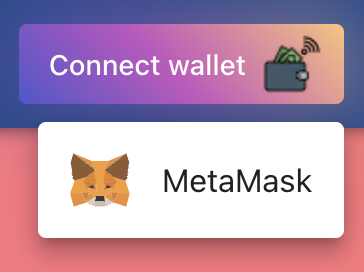
\includegraphics[width=5cm]{img/results/auth-wallet-list.png}
\caption[Insurechain: Available wallets]{\footnotesize{Available wallets.}}
\label{fig:wallet-list}
\end{figure}

When selecting Metamask, a new pop-up will raise to provide permissions to the web app for accessing the wallet data as shown in figure \ref{fig:grant-permission-to-wallet}.

\begin{figure}[H]
\centering
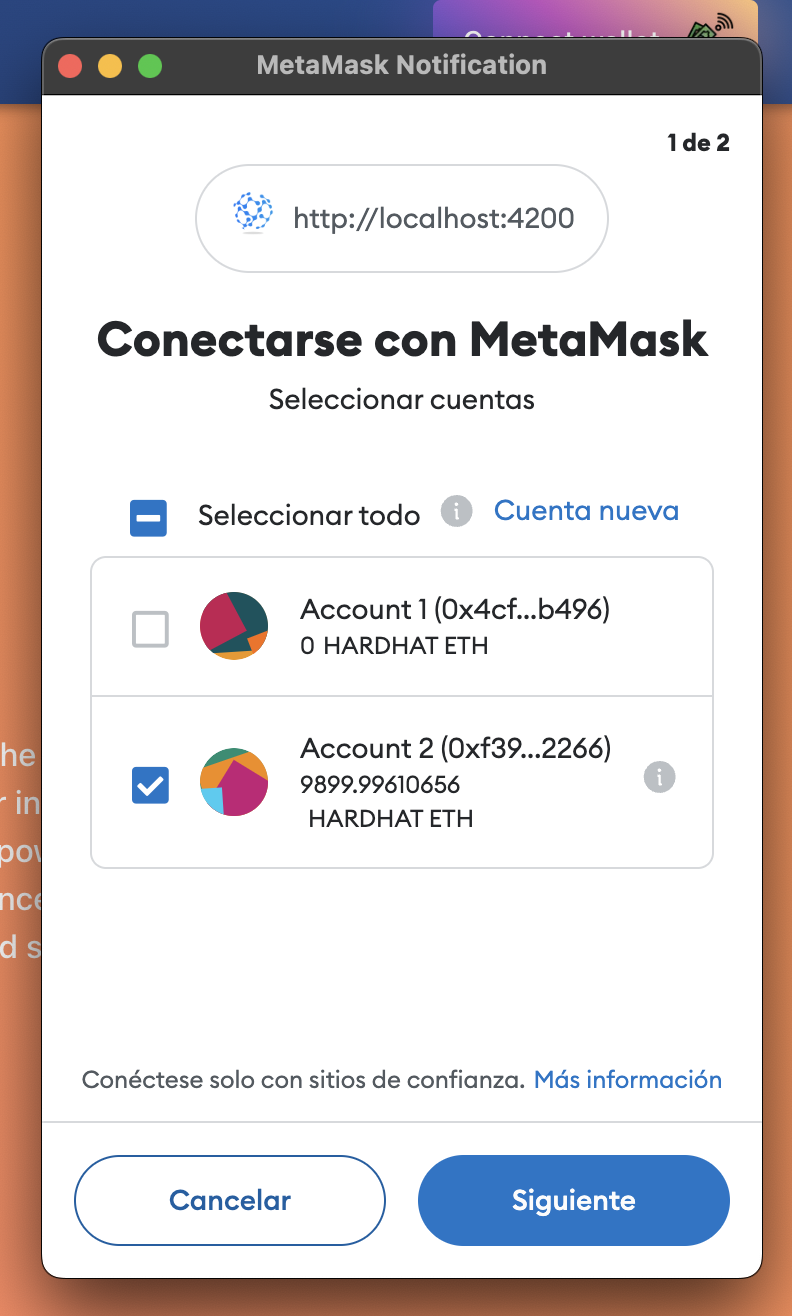
\includegraphics[width=6cm]{img/results/auth-metamask-connect.png}
\caption[Insurechain: Metamask granting access to selected accounts ]{\footnotesize{Metamask granting access to selected accounts}}
\label{fig:grant-permission-to-wallet}
\end{figure}

Once the user has granted the permissions to the app to consume the wallet account data, the frontend immediately requests a nonce to the backend and displays a modal where the user is asked to confirm the signing message as you can see in figure \ref{fig:metamask-sign-in}.

\begin{figure}[H]
\centering
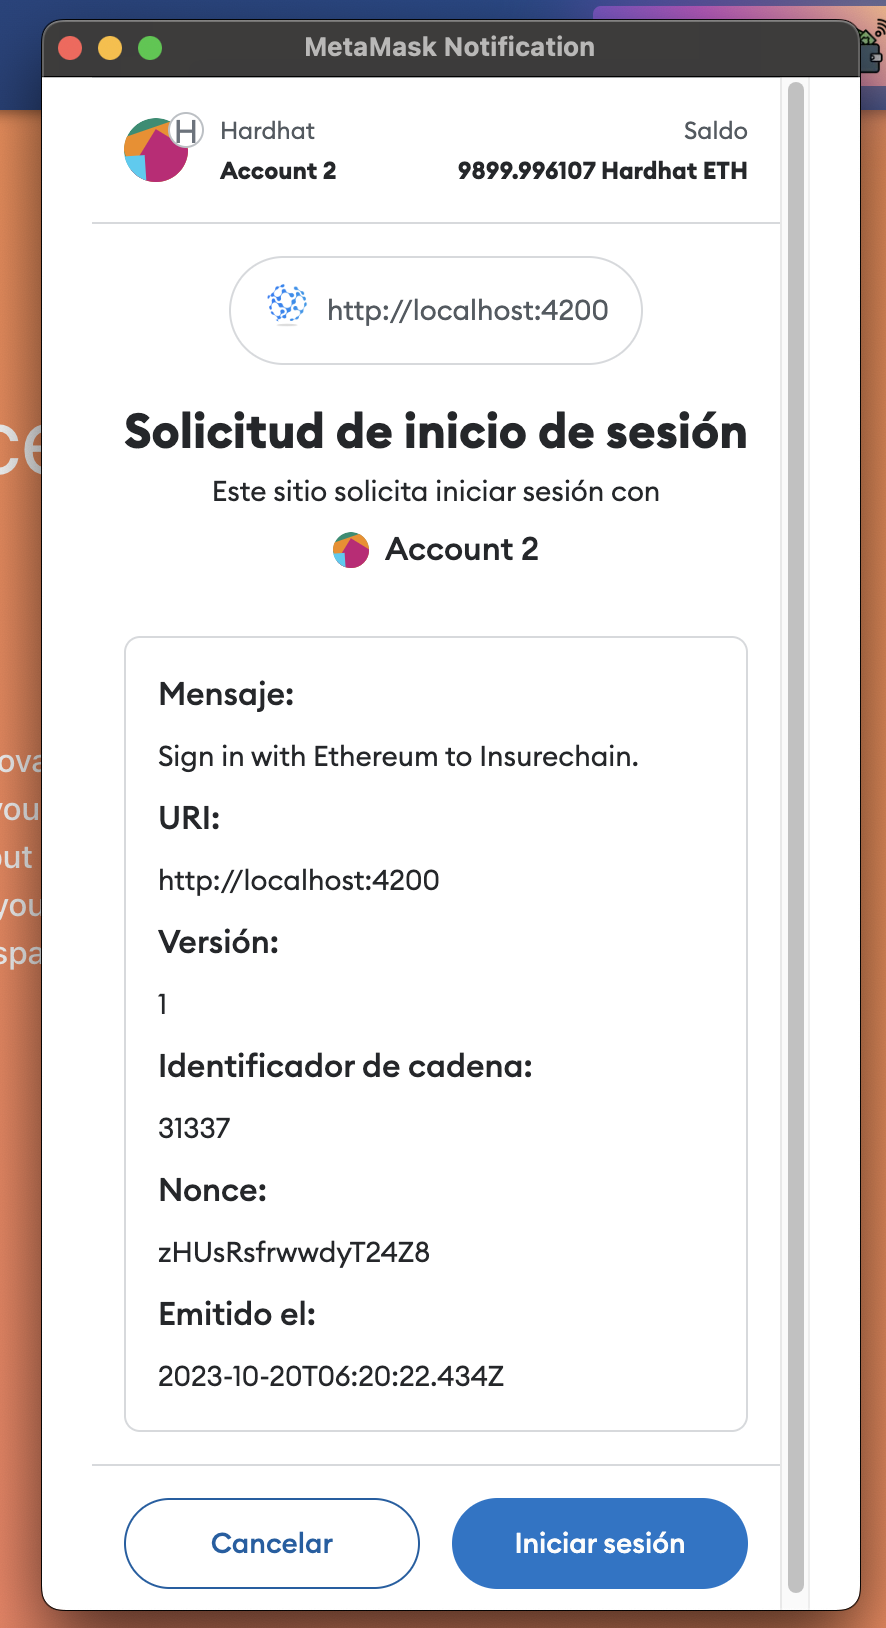
\includegraphics[width=6cm]{img/results/auth-sign-in.png}
\caption[Insurechain: Metamask prompting to sign the sign-in message ]{\footnotesize{Metamask prompting to sign the sign-in message.}}
\label{fig:metamask-sign-in}
\end{figure}

If the user accepts, the message signed is sent to the backend where it verifies it, and if all proceeds as expected, the user gets authenticated so the web displays a notification toast, like the one in figure \ref{fig:auth-success-notification}.

\begin{figure}[H]
\centering
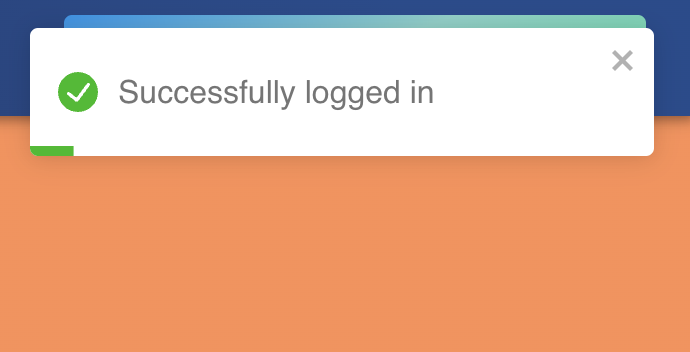
\includegraphics[width=4cm]{img/results/auth-success-notification.png}
\caption[Insurechain: Notification when login succeeds ]{\footnotesize{Notification when login succeeds.}}
\label{fig:auth-success-notification}
\end{figure}

Now, as is represented in figure \ref{fig:header-signed-in}, the header toolbar updates its layout in order to display the first and last characters of the account signed in. This is useful since a user may have several accounts.

\begin{figure}[H]
\centering

\includegraphics[width=12cm]{img/results/header-signedIn.png}
\caption[Insurechain: Header when user sign in succeeds ]{\footnotesize{Toolbar when user sign in succeeds.}}
\label{fig:header-signed-in}
\end{figure}

When clicking this new element, a modal appears to display some information retrieved from the connected wallet. In addition, a button to get disconnected when the user desires and another button to copy the full account address is rendered. You may find it in figure \ref{fig:signed-in-modal}.

\begin{figure}[H]
\centering
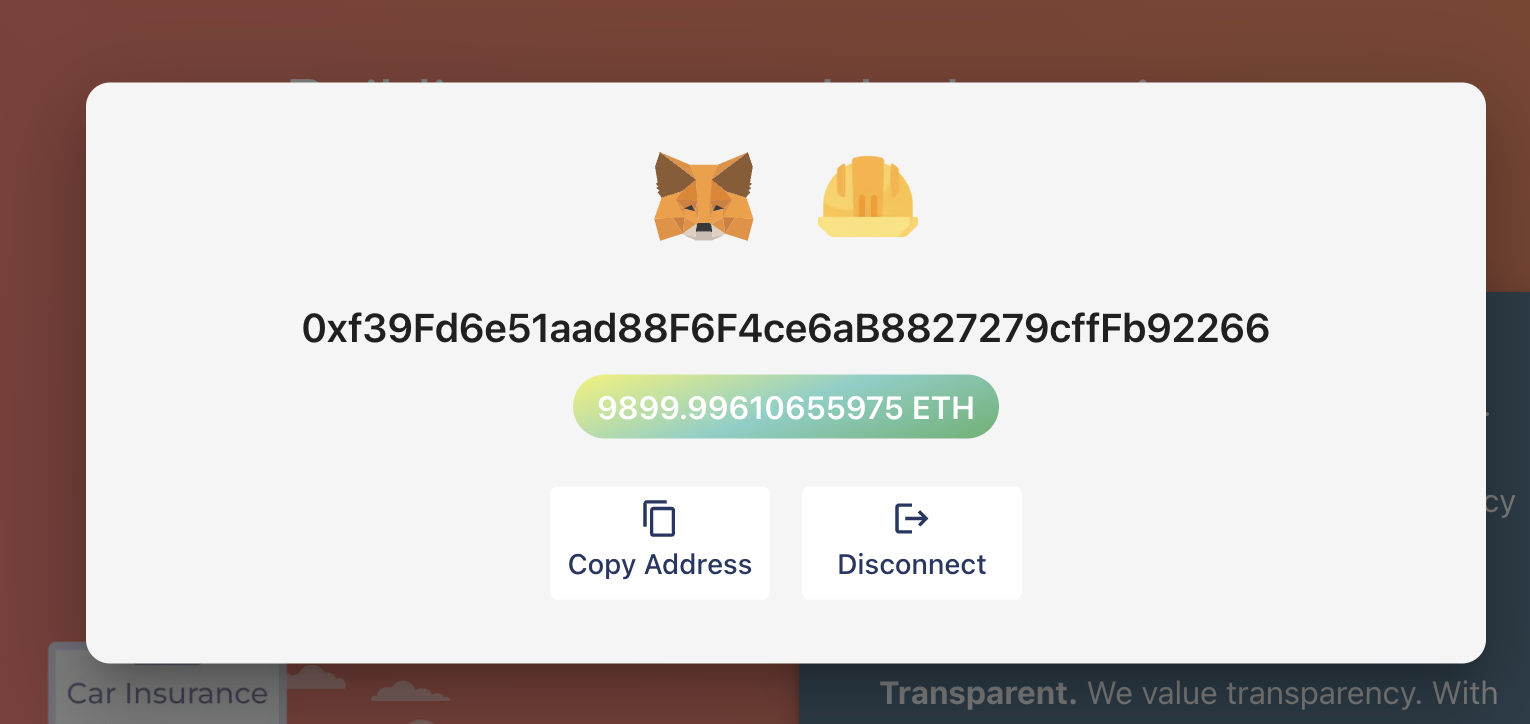
\includegraphics[width=6cm]{img/results/auth-signed-in-modal.png}
\caption[Insurechain: User account modal ]{\footnotesize{User account modal.}}
\label{fig:signed-in-modal}
\end{figure}
}

\subsubsection{Creating a proposal}
{
The user can access the signed-in or not to the insurance contraction page. There, he may find a first form where the user has to introduce all the data about the car to be covered as presented in figure \ref{fig:checkout-car-form}.

\begin{figure}[H]
\centering
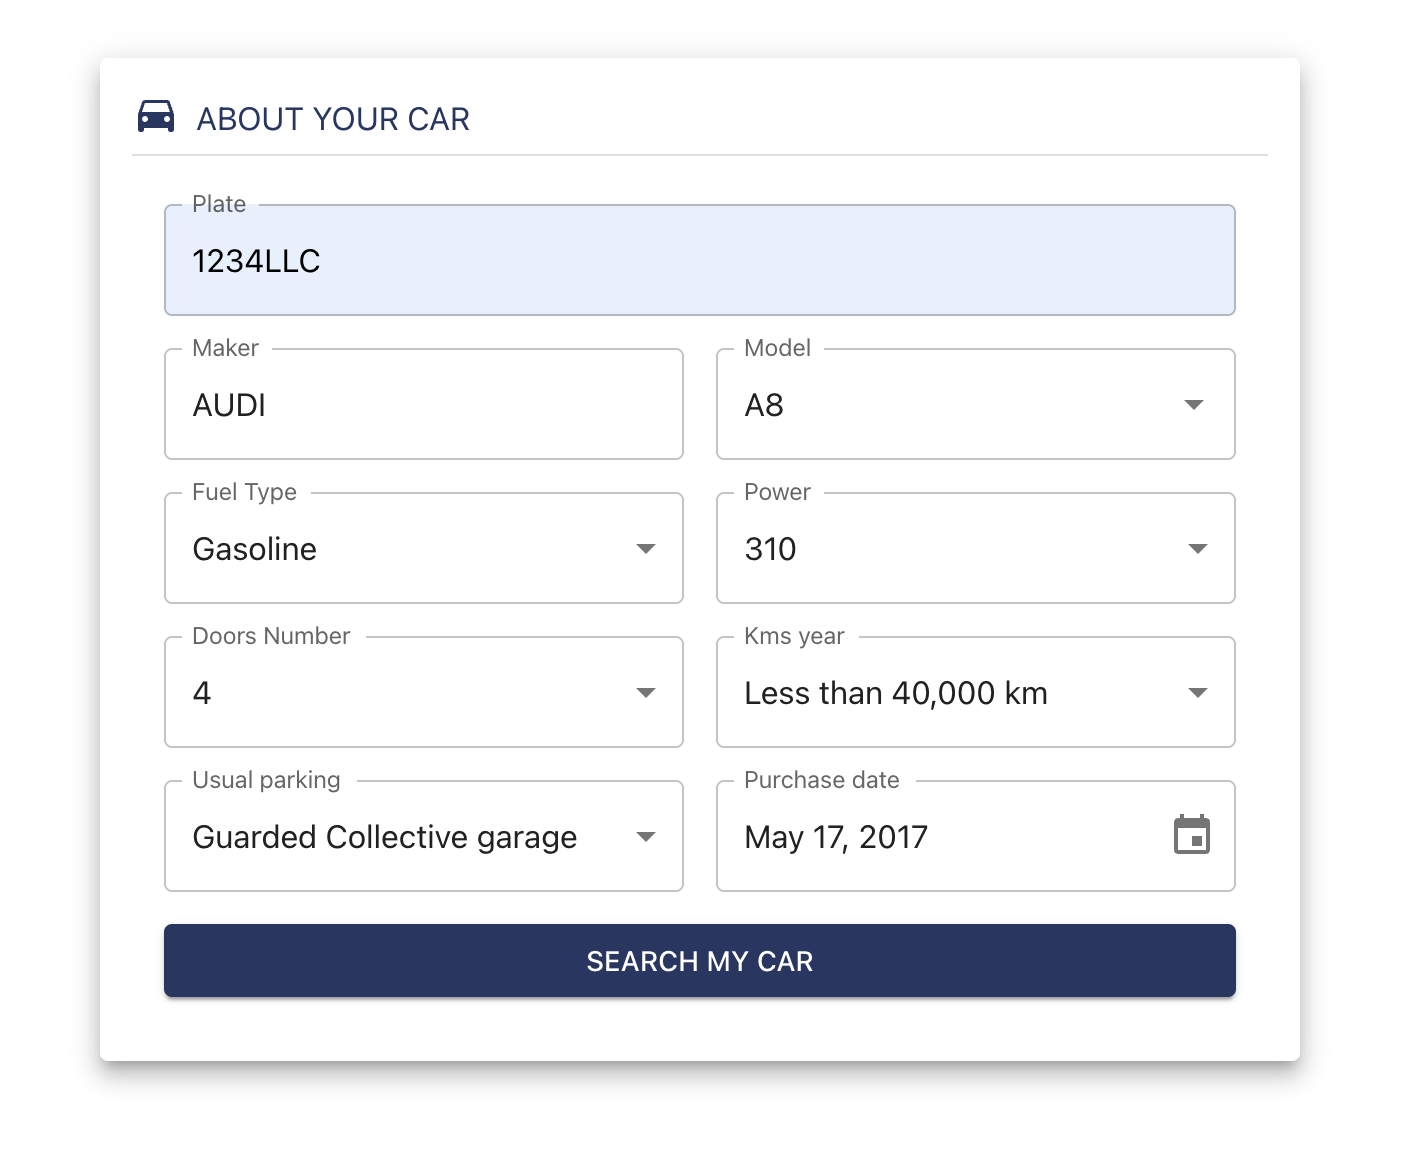
\includegraphics[width=10cm]{img/results/checkout-car.png}
\caption[Insurechain: Car form insurance enrollment]{\footnotesize{Car form insurance enrollment.}}
\label{fig:checkout-car-form}
\end{figure}
Then, the user must select the specific version for the car detailed as is demonstrated in figure \ref{fig:checkout-select-version}. These car models are consumed for a public API.

\begin{figure}[H]
\centering
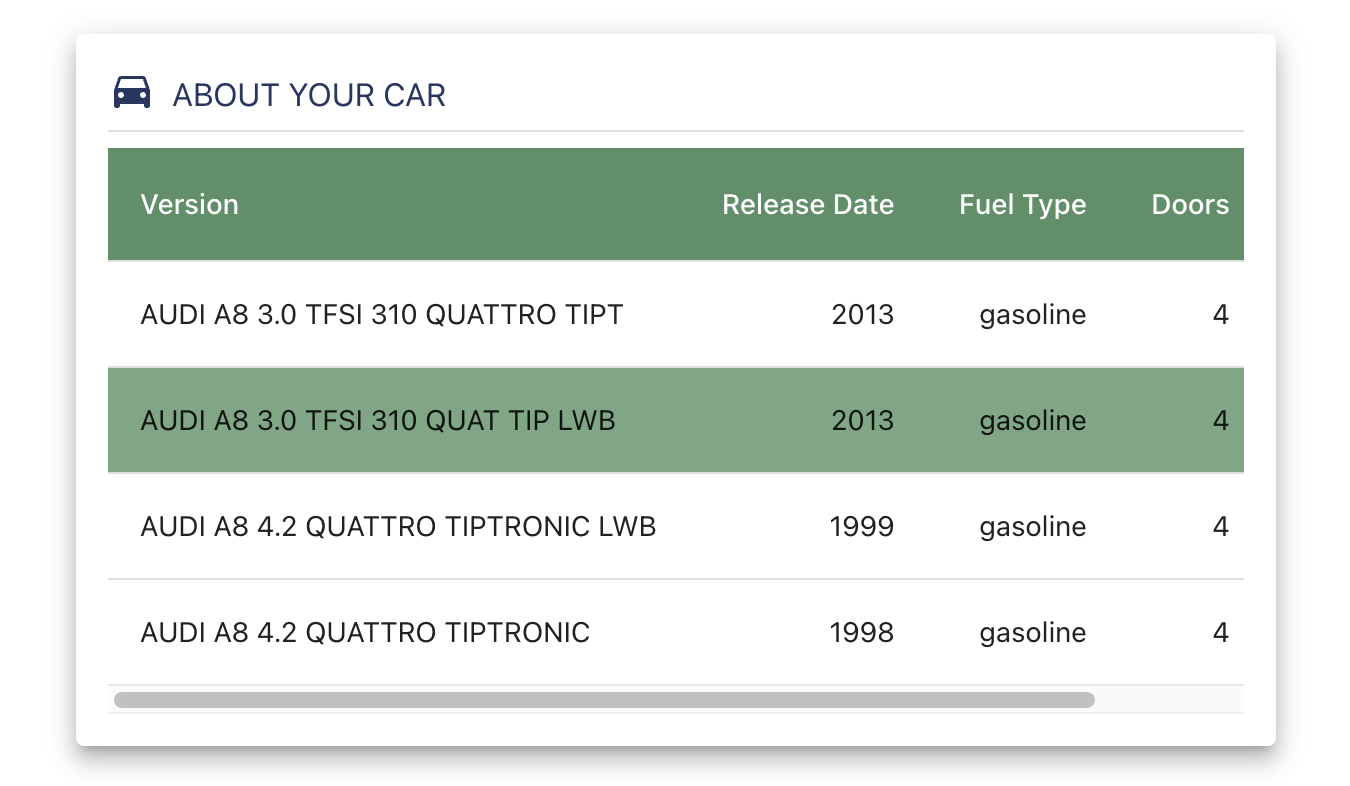
\includegraphics[width=10cm]{img/results/checkout-select-version.png}
\caption[Insurechain: Car version selection in insurance enrollment]{\footnotesize{Car version selection in insurance enrollment.}}
\label{fig:checkout-select-version}
\end{figure}

With the specific version and model of the car defined, the app displays a form to ask for the driver's information. Note in figure \ref{fig:checkout-driver-form} that the car information is collected and displayed in the first block above the driver's form.

\begin{figure}[H]
\centering
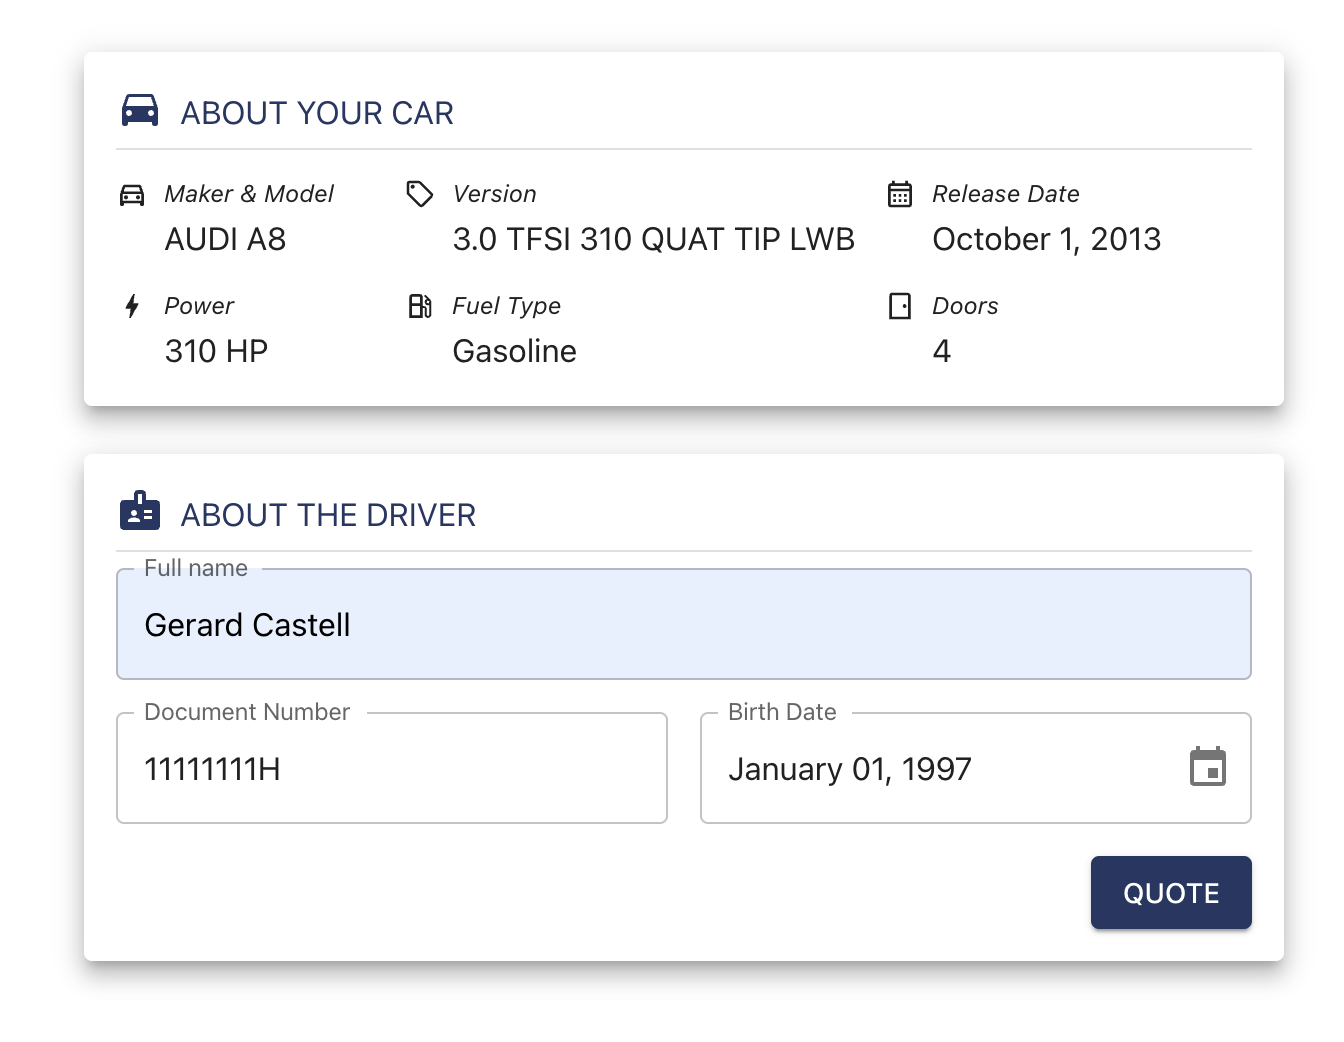
\includegraphics[width=10cm]{img/results/checkout-about-you.png}
\caption[Insurechain: Driver form in insurance enrollment]{\footnotesize{Driver form in insurance enrollment.}}
\label{fig:checkout-driver-form}
\end{figure}

With all this information introduced, a summary of such risk figures is displayed on top as shown in figure \ref{fig:checkout-coverage-selection}, the web app makes a quote and the backend calculates a price for each coverage type. This price is random since it is out of the scope of the project. Thus, the backend server returns all the coverage products with a monthly price associated and the web displays it. Note that the price is reflected in euros and \acrshort{eth}. This conversion is obtained in real time to a public API.

\begin{figure}[H]
\centering
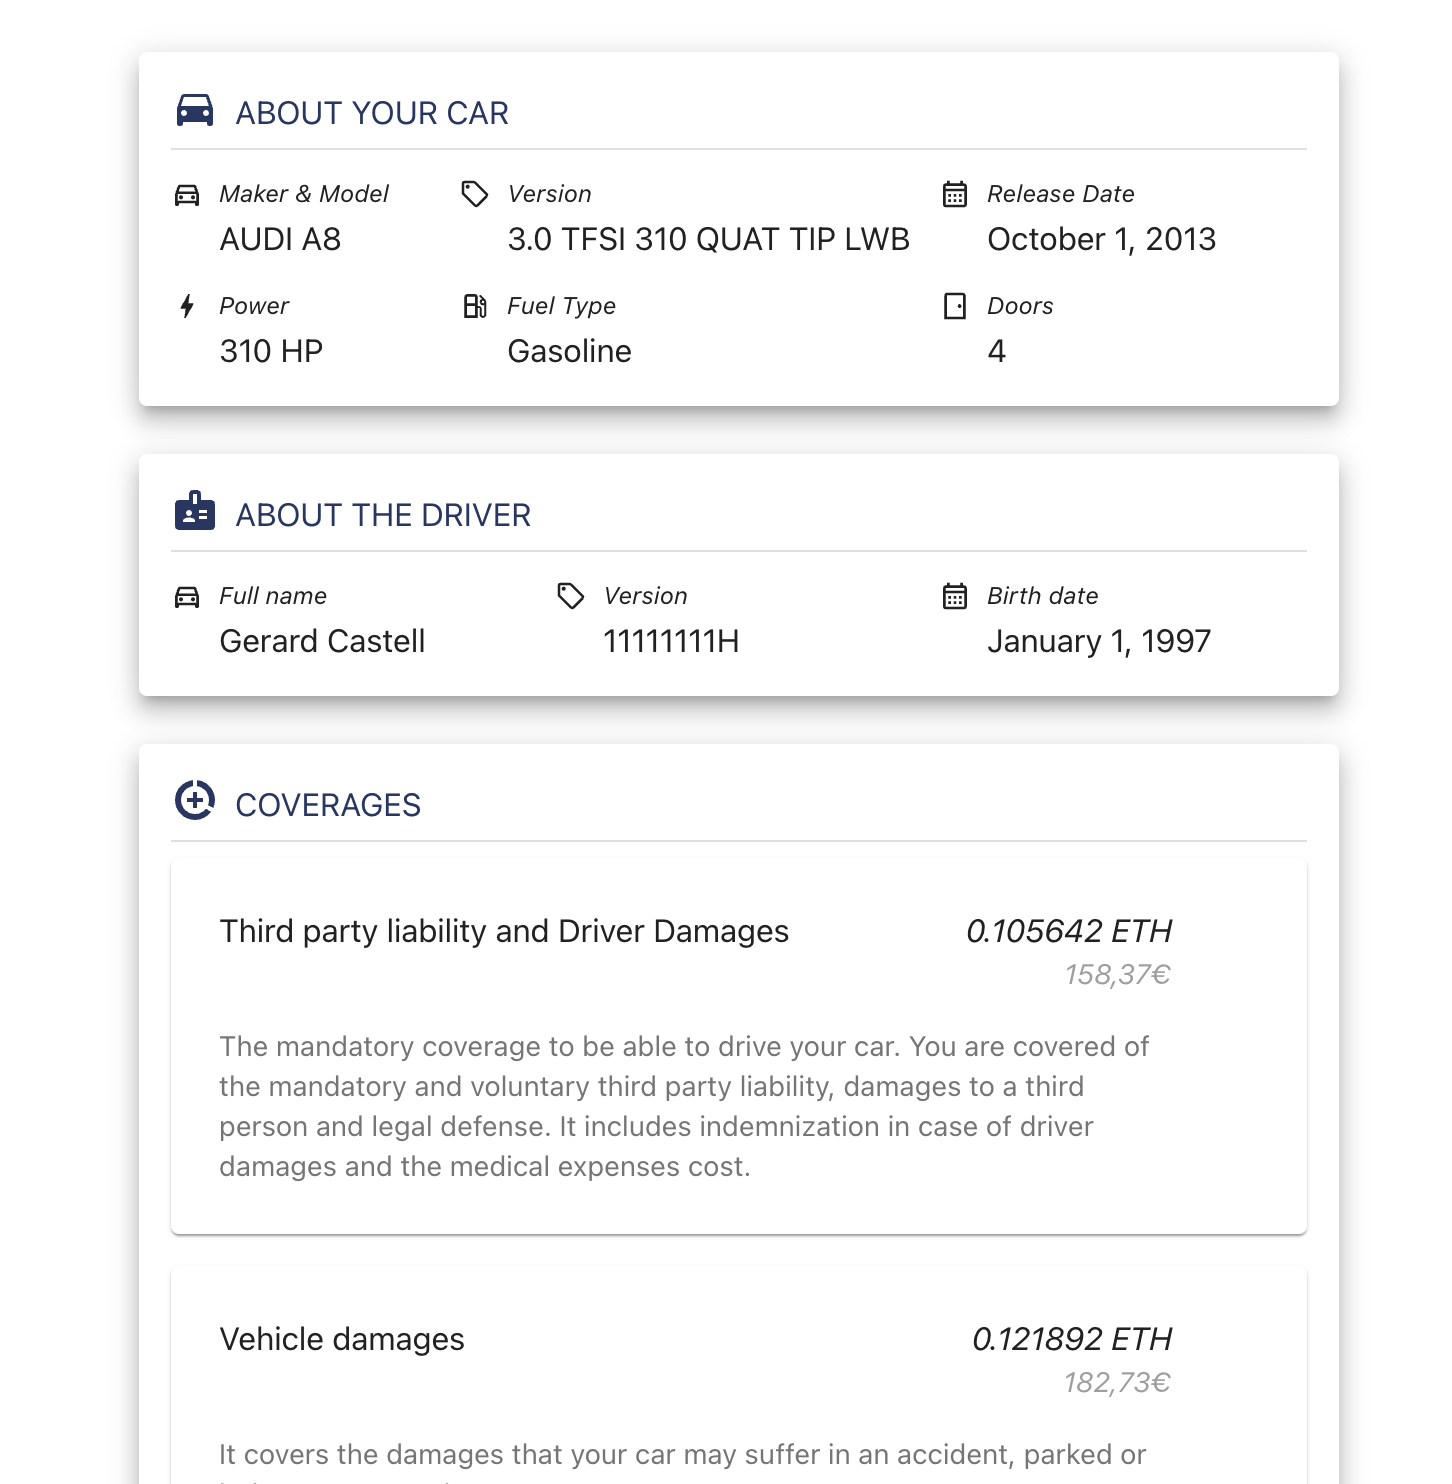
\includegraphics[width=10cm]{img/results/checkout-coverage-selection.png}
\caption[Insurechain: Risk figures summary in insurance enrollment]{\footnotesize{Risk figures summary in insurance enrollment.}}
\label{fig:checkout-coverage-selection}
\end{figure}

The user can select the coverage types in which he is interested and then save the proposal when he is ready as illustrated in figure \ref{fig:checkout-coverage-selection-2}.

\begin{figure}[H]
\centering
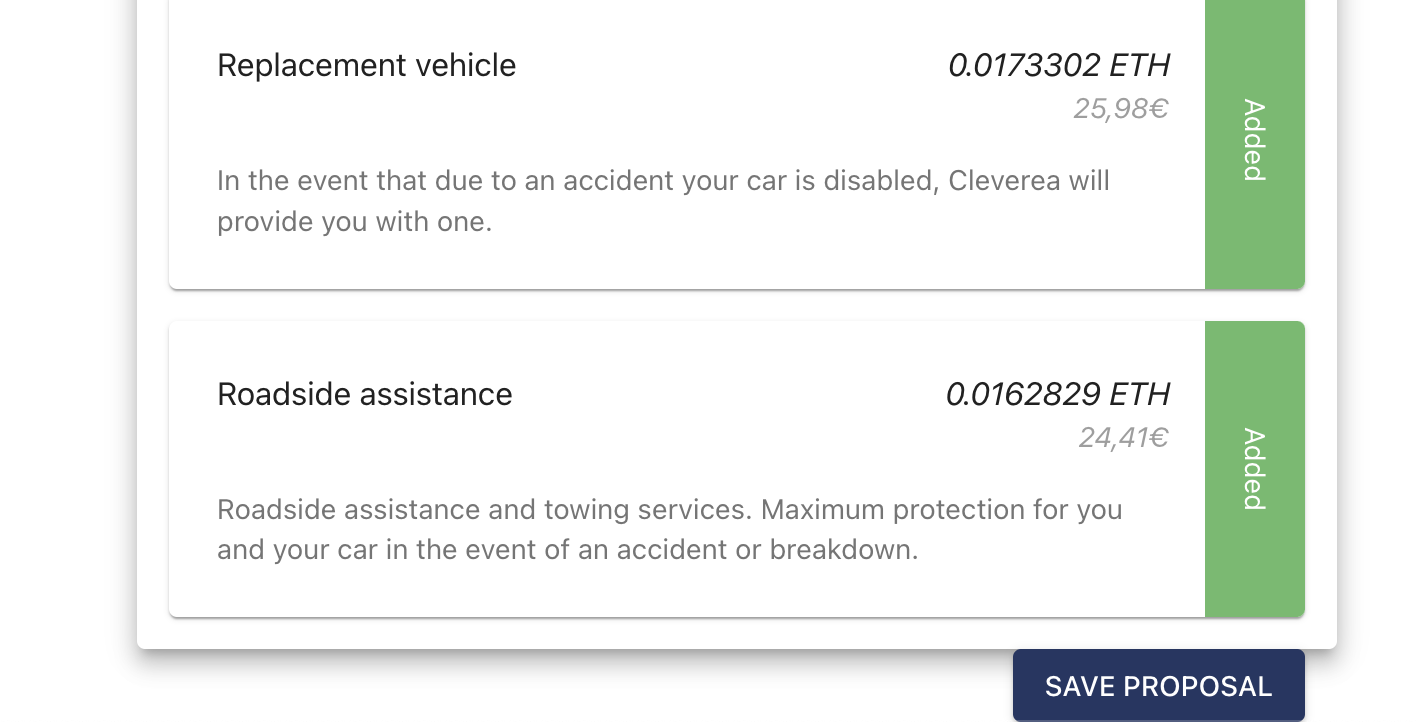
\includegraphics[width=10cm]{img/results/checkout-coverage-selection-2.png}
\caption[Insurechain: Coverage types selection in insurance enrollment]{\footnotesize{Coverage types selection in insurance enrollment.}}
\label{fig:checkout-coverage-selection-2}
\end{figure}

Eventually, when the user wants to confirm it has to be signed in. Otherwise, a modal like the one in figure \ref{fig:metamask-sign-in} will appear. Once logged in, the web app sends the proposal configuration with the risk figures data to the backend with the authentication header. The backend stores the proposal bound to that client in the database and returns an OK. Consequently, the web displays a modal announcing the confirmation as you can see in figure \ref{fig:checkout-succeed-modal}.

\begin{figure}[H]
\centering
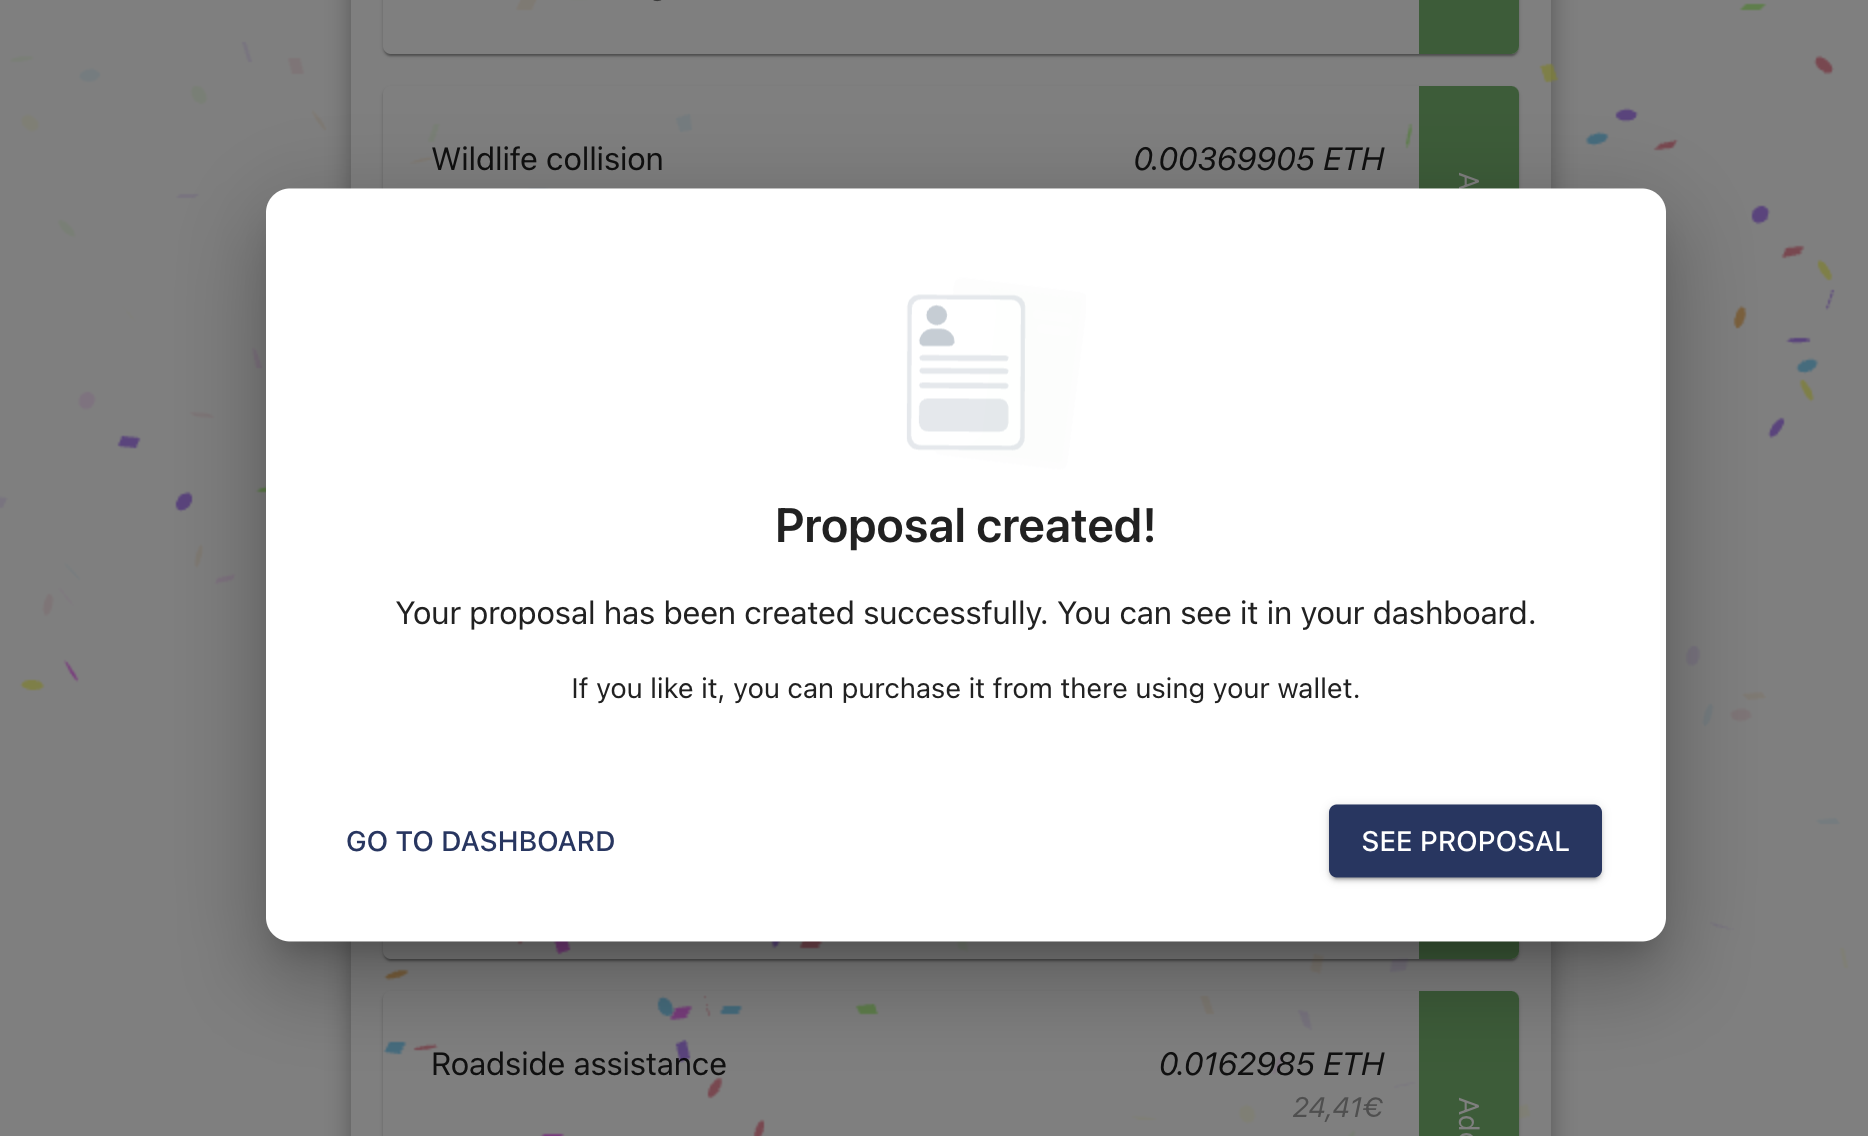
\includegraphics[width=10cm]{img/results/checkout-succeed.png}
\caption[Insurechain: Succeed modal in insurance enrollment]{\footnotesize{Succeed modal in insurance enrollment.}}
\label{fig:checkout-succeed-modal}
\end{figure}
}

\subsubsection{Show user proposals}
{
If the user wants to see their proposals he can access them on the dashboard page, where he may find two boxes to visit existing proposals or policies as revealed in figure \ref{fig:dashboard-page}.

\begin{figure}[H]
\centering
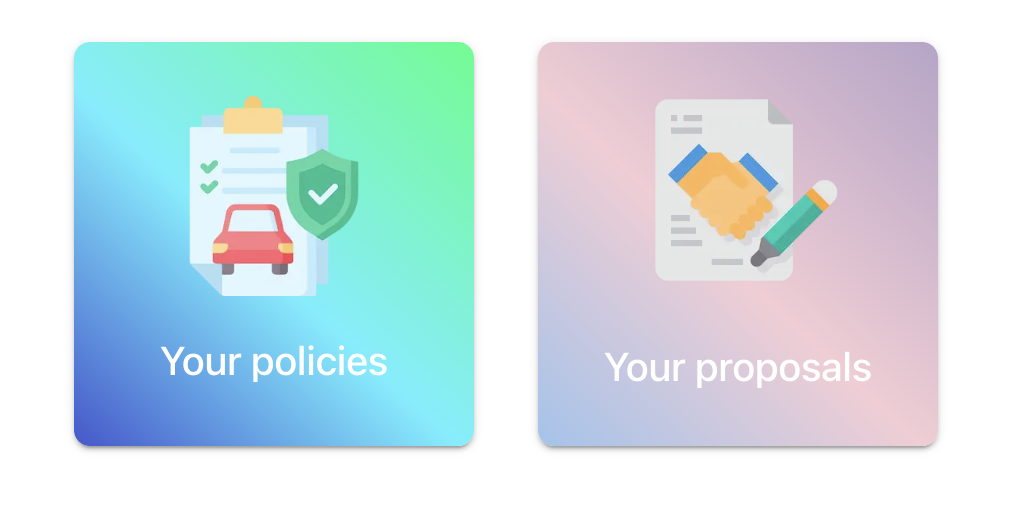
\includegraphics[width=8cm]{img/results/dashboard.png}
\caption[Insurechain: Dashboard page]{\footnotesize{Dashboard page.}}
\label{fig:dashboard-page}
\end{figure}

If the user selects proposals, the user proposals page will appear as in the figure \ref{fig:proposals-page}.
On this page, the user may find all his proposals, purchased and still not, listed with a summary of this accorded data and price.

\begin{figure}[H]
\centering
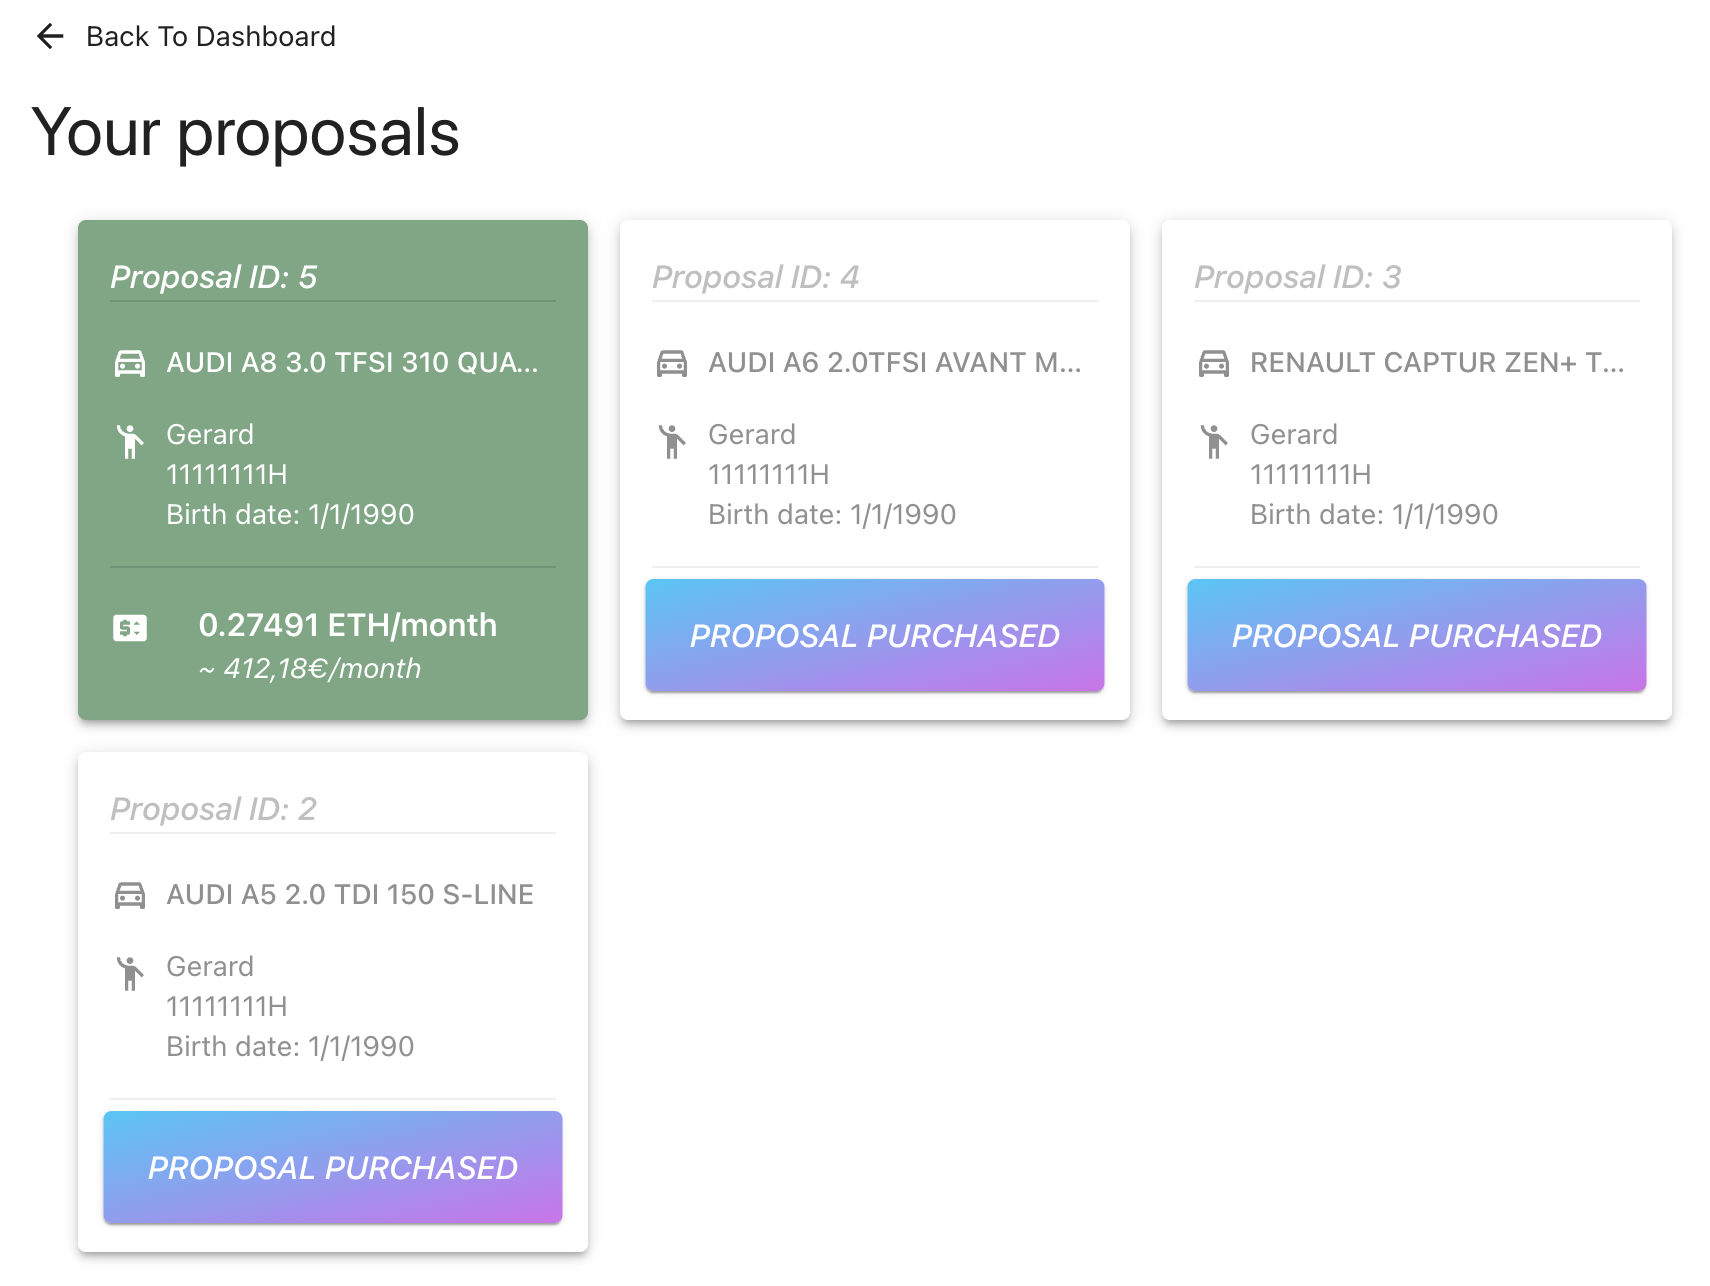
\includegraphics[width=12cm]{img/results/proposals-list.png}
\caption[Insurechain: Proposals page]{\footnotesize{Proposals page.}}
\label{fig:proposals-page}
\end{figure}

If the user selects the first one which is the last one created he will navigate to the detail of such proposal as reflected in figure \ref{fig:proposal-detail}.
\begin{figure}[H]
\centering
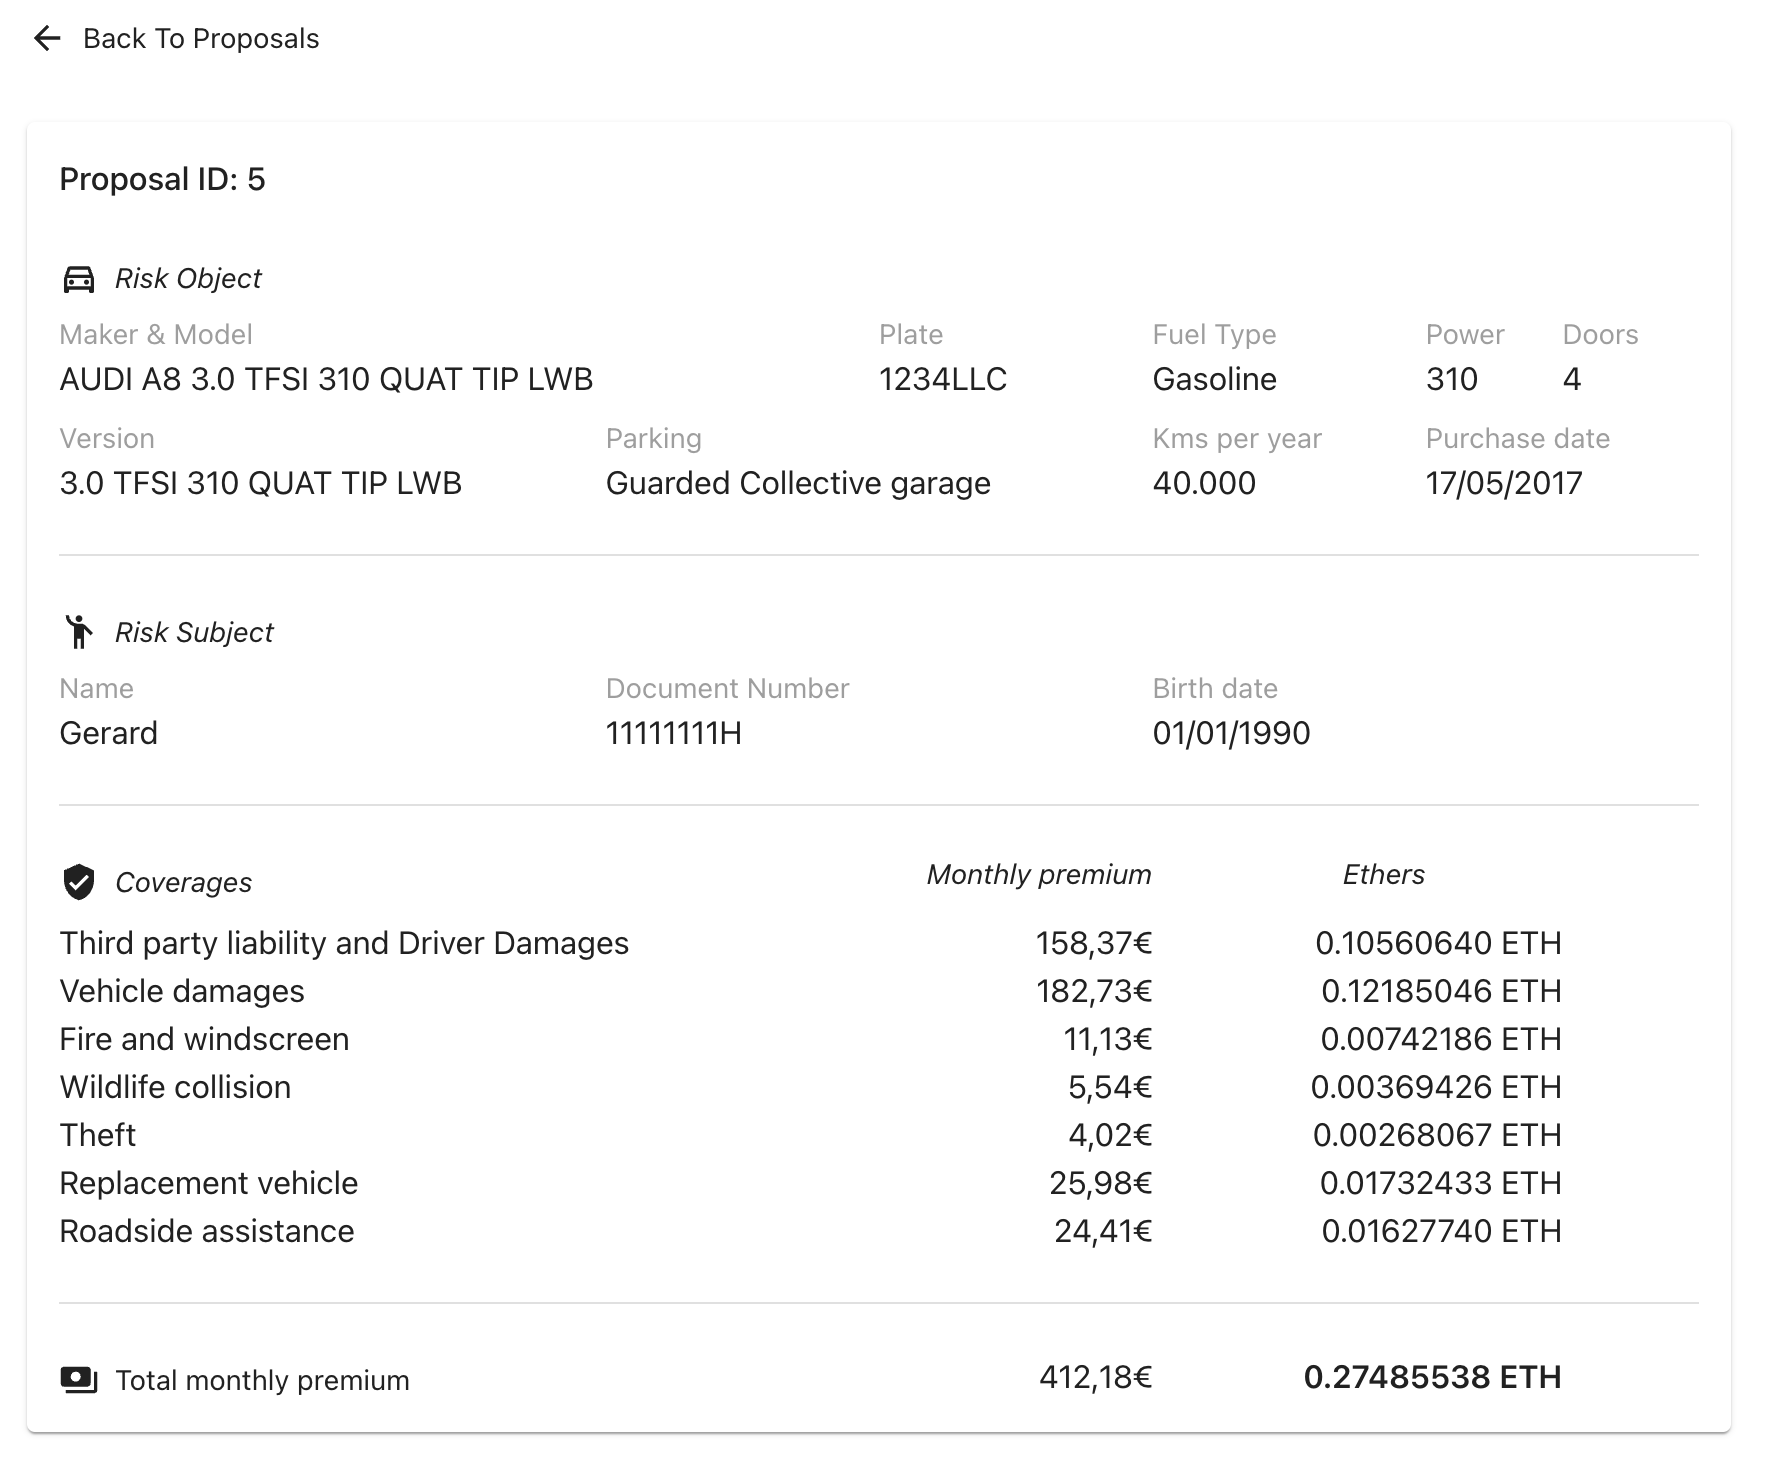
\includegraphics[width=12cm]{img/results/proposal-detail-1.png}
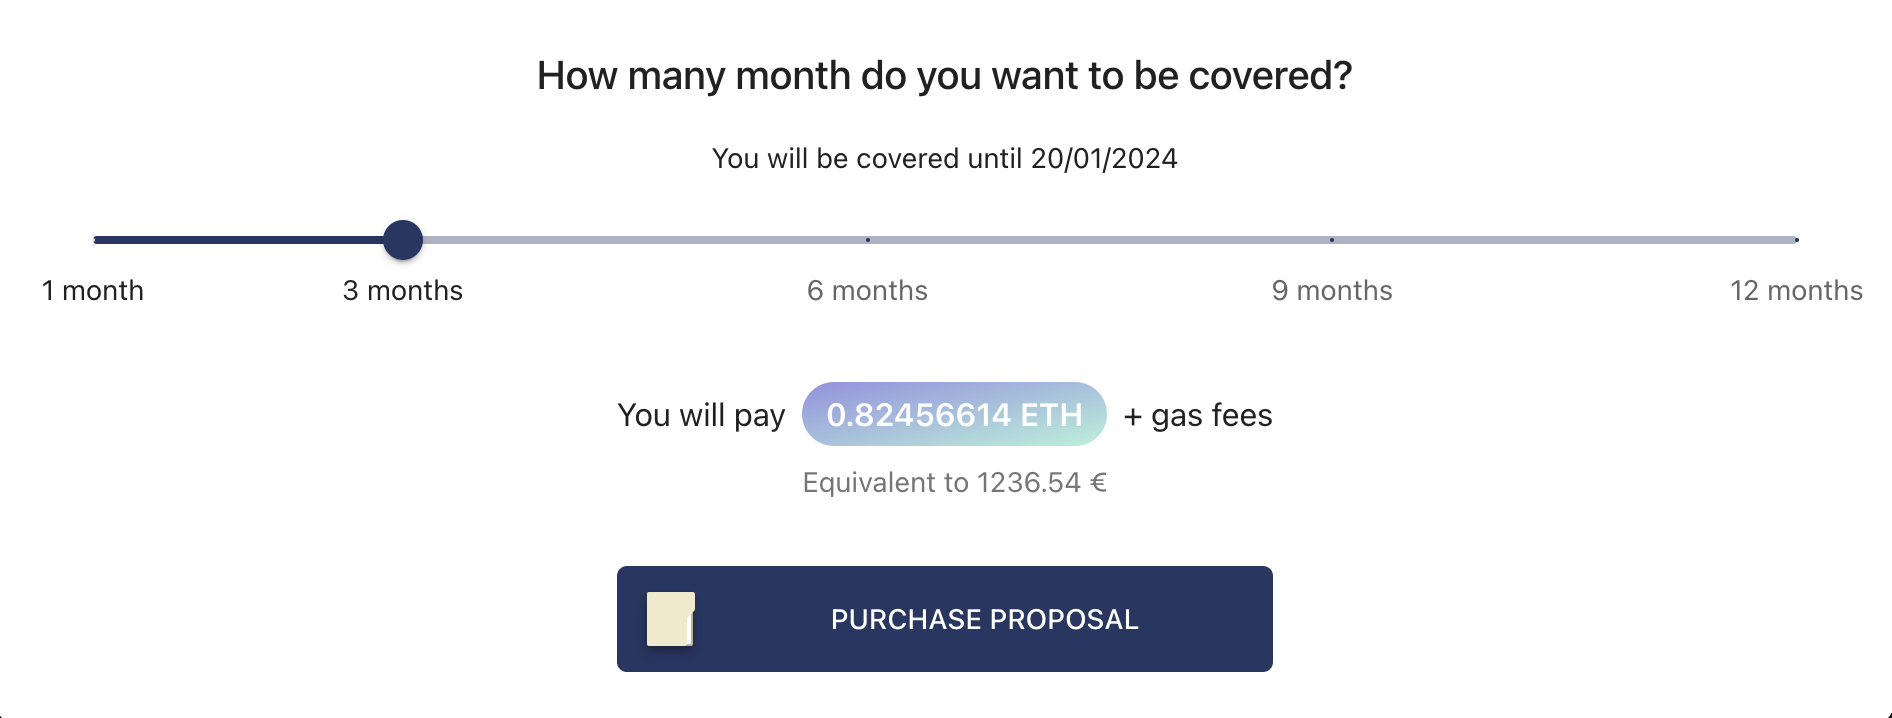
\includegraphics[width=12cm]{img/results/proposal-detail-2.png}
\caption[Insurechain: Proposal detail page]{\footnotesize{Proposal detail page.}}
\label{fig:proposal-detail}
\end{figure}

The web requests the backend for the specific proposal and it is returned. Then the user may find on this page all the proposal information collected on the proposal form. It is important to focus that for purchase the user must select the number of months to be covered from the current day. The total monthly amount will be multiplied by the number of months and this total price is indicated at the bottom. Take into account that this is a rough calculation because the \acrshort{eth} cannot be accurate at that moment and the gas needed to purchase the policy is not estimated.
}

\subsubsection{Purchase proposal}
\label{section:purchase-proposal}
{
In the proposal detail page, when the user clicks the purchase proposal button the wallet will display a confirmation of the according transaction as shown in figure \ref{fig:purchase-transaction}.

\begin{figure}[H]
\centering
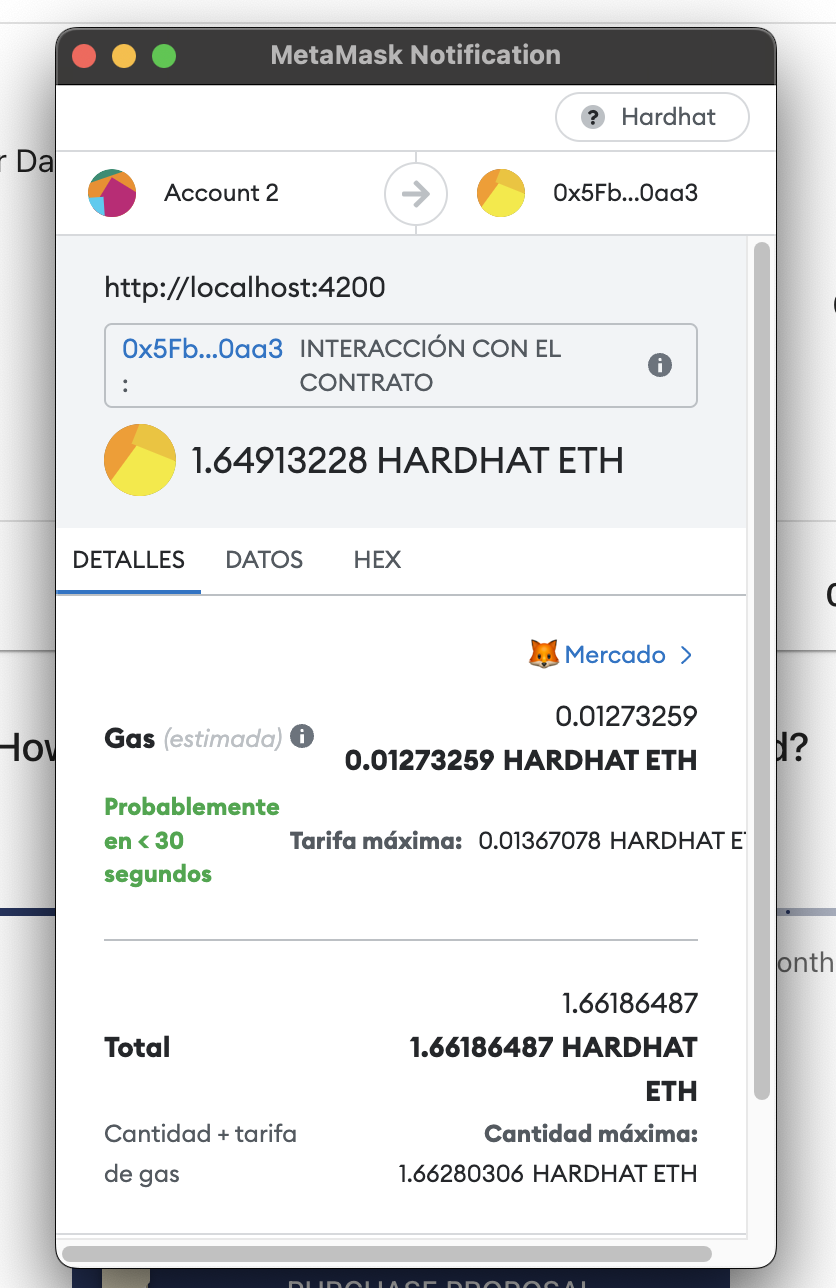
\includegraphics[width=6cm]{img/results/purchase-transaction.png}
\caption[Insurechain: Purchase transaction]{\footnotesize{Purchase transaction.}}
\label{fig:purchase-transaction}
\end{figure}


If the user agrees, the transaction will be sent to the factory smart contracts. If the computation succeeds a modal will be displayed as you may see in figure \ref{fig:purchase-succeed-modal}. 

\begin{figure}[H]
\centering
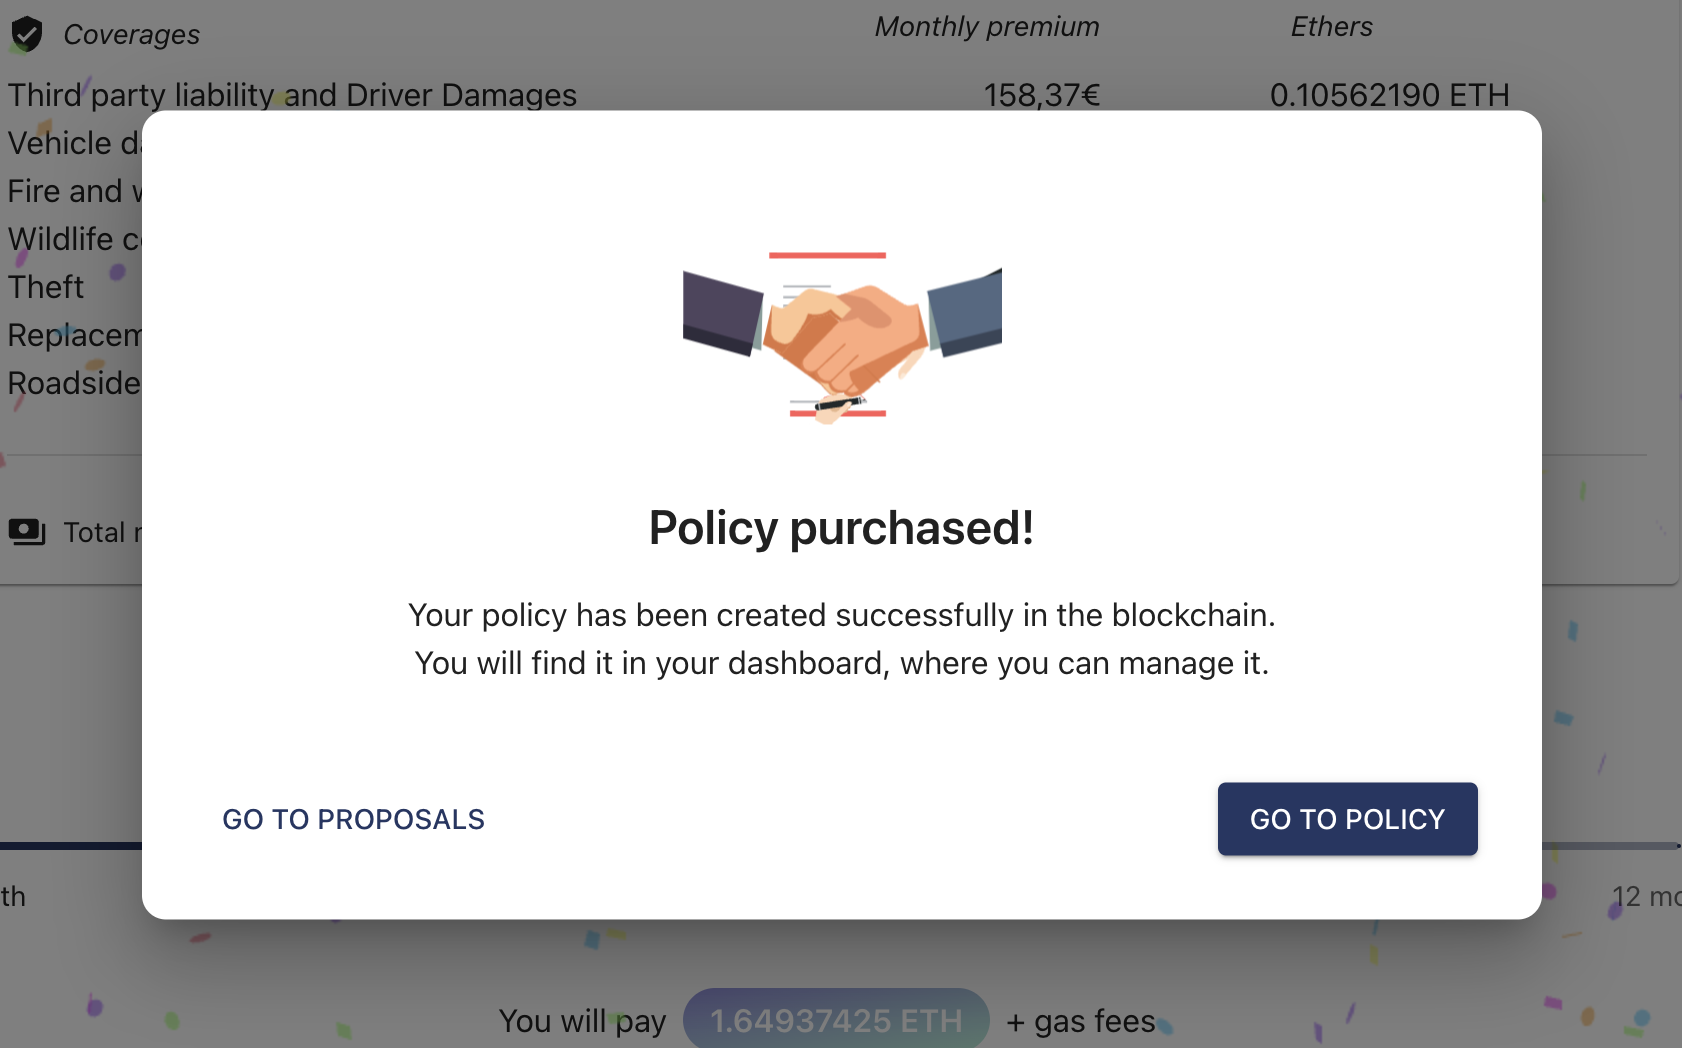
\includegraphics[width=10cm]{img/results/purchase-succeed-modal.png}
\caption[Insurechain: Purchase succeed modal]{\footnotesize{Purchase succeed modal.}}
\label{fig:purchase-succeed-modal}
\end{figure}
Keep in mind, that the transaction has proceeded successfully, however, to consider the transaction as confirmed and make sure the data can be considered immutable in the Ethereum blockchain we must way a few blocks yet. If we evaluate the Metamask within that period of time we will see something similar to the figure \ref{fig:pending-transaction}.

\begin{figure}[H]
\centering
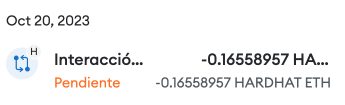
\includegraphics[width=6cm]{img/results/transaction-pending.png}
\caption[Insurechain: Transaction pending]{\footnotesize{Transaction pending.}}
\label{fig:pending-transaction}
\end{figure}
Eventually, when the wallet considers that enough blocks have been mined and the state is immutable the transaction turns confirmed as you can see in figure \ref{fig:confirmed-transaction}.

\begin{figure}[H]
\centering
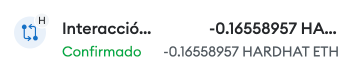
\includegraphics[width=6cm]{img/results/transaction-confirmed.png}
\caption[Insurechain: Transaction confirmed]{\footnotesize{Transaction confirmed.}}
\label{fig:confirmed-transaction}
\end{figure}
}

\subsubsection{Show user policies}
{
The user will find all the policies purchased and canceled on the policies page as illustrated in figure \ref{fig:policies-page}.

\begin{figure}[H]
\centering
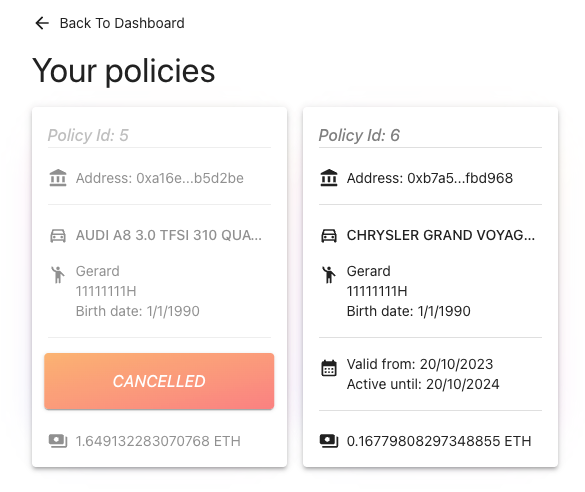
\includegraphics[width=8cm]{img/results/policies-page.png}
\caption[Insurechain: Policies page]{\footnotesize{Policies page.}}
\label{fig:policies-page}
\end{figure}

If we visit the policy purchased before, we have to see exactly the same data that was reflected in the proposal page but with the difference that now the source is the Policy smart contract deployed in the purchase and not the backend database. The total amount paid must be different because the price displayed is precisely the paid in the purchase transaction that was stored in the policy smart contract. This data comparison can be performed by comparing figures \ref{fig:proposal-detail} and \ref{fig:policy-detail}.

\begin{figure}[H]
\centering
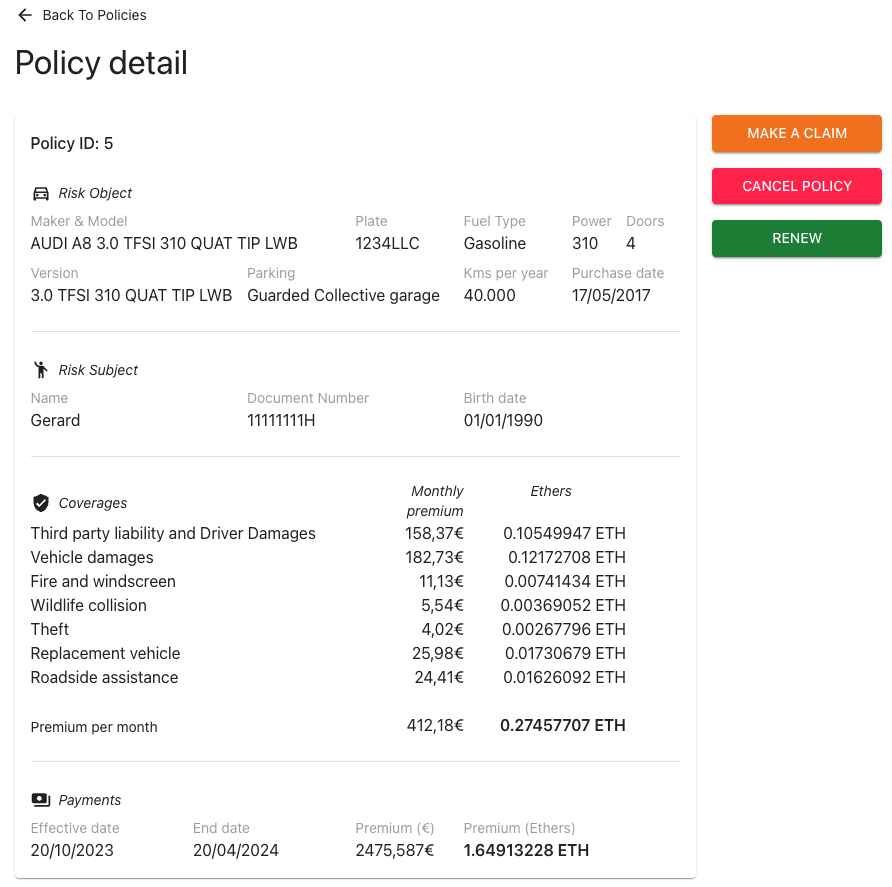
\includegraphics[width=12cm]{img/results/policy-detail.png}
\caption[Insurechain: Policy detail page]{\footnotesize{Policy detail page.}}
\label{fig:policy-detail}
\end{figure}

}

\subsubsection{Cancel policy}
{
Furthermore, if we look at the right side we find three buttons to make a claim, renew and cancel. Just the cancel button is implemented as explained before. If we press this button, the web app estimates how much \acrshort{eth} would be refunded to the user according to the time not consumed of the policy live as observed in the figure \ref{fig:cancel-modal}.

\begin{figure}[H]
\centering
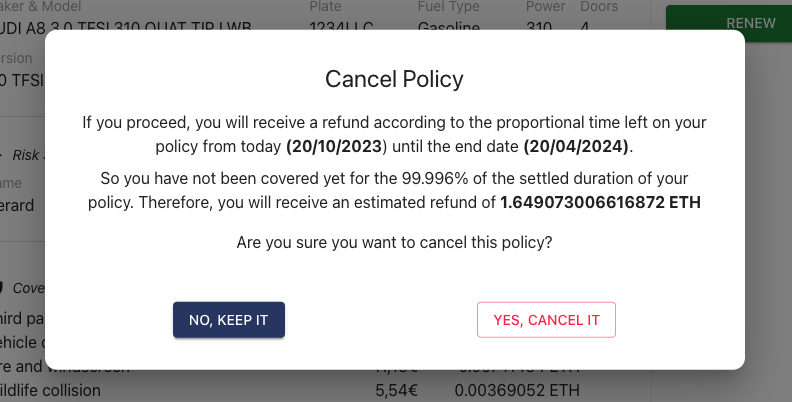
\includegraphics[width=9cm]{img/results/cancel-modal.png}
\caption[Insurechain: Cancel policy prompt modal]{\footnotesize{Cancel policy prompt modal.}}
\label{fig:cancel-modal}
\end{figure}

If the user confirms the modal, the wallet will trigger a transaction modal to confirm the gas spent as you may see in figure \ref{fig:cancel-transaction}. This is due to the user is going to modify the state of the policy contract since some store variables are going to change their value such as the end date or the renewal date. The amount of \acrshort{eth} is not too high so it is reasonable that this charge falls on the client side.

\begin{figure}[H]
\centering
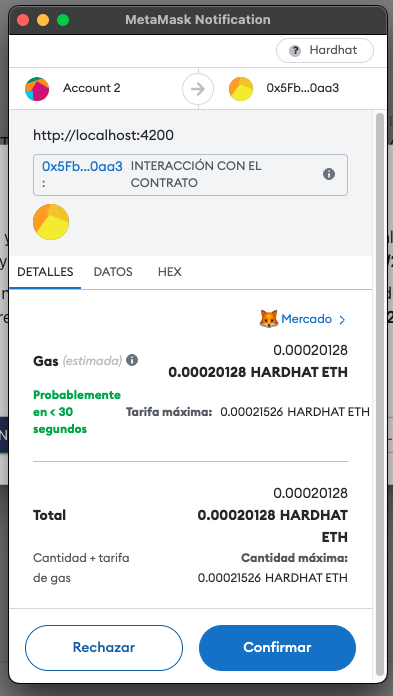
\includegraphics[width=6cm]{img/results/cancel-transaction.png}
\caption[Insurechain: Cancel policy transaction]{\footnotesize{Cancel policy transaction.}}
\label{fig:cancel-transaction}
\end{figure}

When the user confirms the transaction if the operation succeeds the user will see the layout displayed in figure \ref{fig:policy-canceled}. Even though, as explained in the section \ref{section:purchase-proposal} the operation has succeeded, nevertheless, to consider the state immutable we must wait for a few transactions.

\begin{figure}[H]
\centering
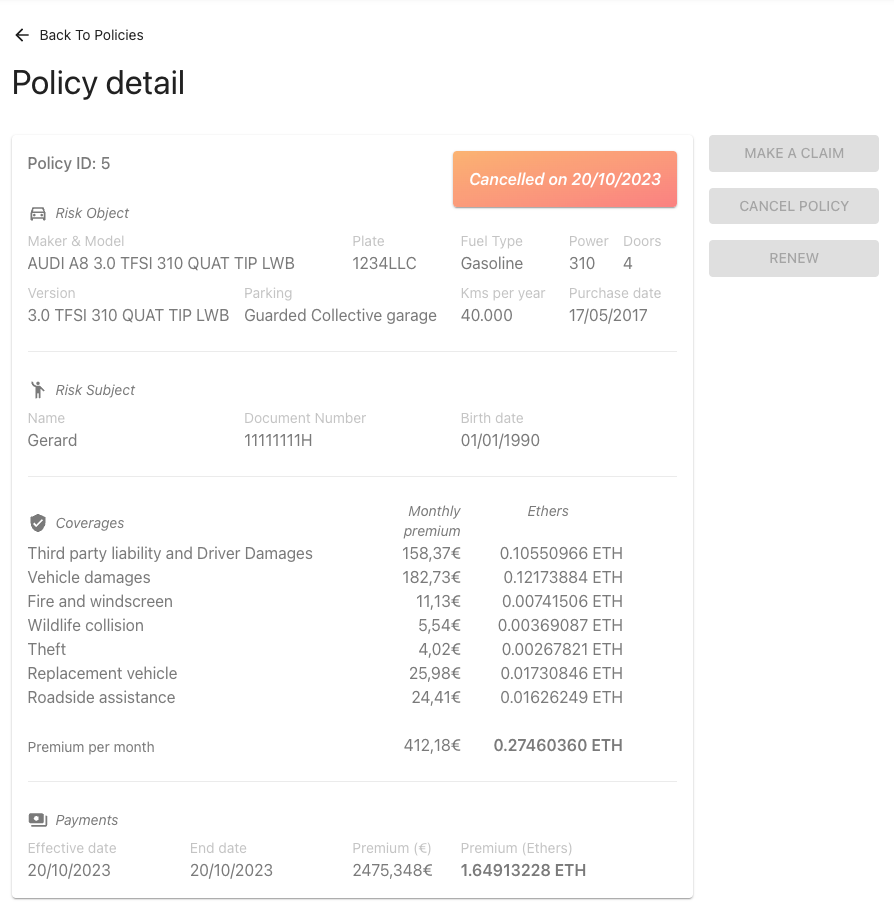
\includegraphics[width=10cm]{img/results/policy-canceled.png}
\caption[Insurechain: Policy canceled page]{\footnotesize{Policy canceled page.}}
\label{fig:policy-canceled}
\end{figure}
}